\documentclass[10pt,a4paper,onecolumn]{article}
% \usepackage[utf8]{inputenc}
\usepackage{marginnote}
\usepackage{graphicx}
\usepackage{xcolor}
\usepackage{authblk,etoolbox}
\usepackage{titlesec}
\usepackage{calc}
\usepackage{hyperref}
\hypersetup{breaklinks=true,
            bookmarks=true,
            pdfauthor=
{
      Metzner Christoph,
  },
            pdftitle=
{
[Re] Modeling GABA Alterations in Schizophrenia: A Link Between Impaired
Inhibition and Gamma and Beta Auditory Entrainment
},
            colorlinks=true,
            citecolor=blue,
            urlcolor=blue,
            linkcolor=blue,
            pdfborder={0 0 0}}
\urlstyle{same}
\usepackage{tcolorbox}
\usepackage{ragged2e}
\usepackage{fontspec}
\usepackage{fontawesome}
\usepackage{caption}
\usepackage{listings}
\lstnewenvironment{code}{\lstset{language=Haskell,basicstyle=\small\ttfamily}}{}

\usepackage{placeins}

%\usepackage{fancyvrb}
%\VerbatimFootnotes
%\usepackage{graphicx}
%\usepackage{mdframed}
%\newmdenv[backgroundcolor=lightgray]{Shaded}


\usepackage{longtable,booktabs}

\usepackage[
  backend=biber,
%  style=alphabetic,
%  citestyle=numeric
]{biblatex}
\bibliography{bibliography.bib}



% --- Macros ------------------------------------------------------------------
\renewcommand*{\bibfont}{\small \sffamily}

\definecolor{red}{HTML}{CF232B}
\newcommand{\ReScience}{Re{\bfseries \textcolor{red}{Science}}}

\newtcolorbox{rebox}
   {colback=blue!5!white, colframe=blue!40!white,
     boxrule=0.5pt, arc=2pt, fonttitle=\sffamily\scshape\bfseries,
     left=6pt, right=20pt, top=6pt, bottom=6pt}

\newtcolorbox{repobox}
   {colback=red, colframe=red!75!black,
     boxrule=0.5pt, arc=2pt, left=6pt, right=6pt, top=3pt, bottom=3pt}

% fix for pandoc 1.14     
\newcommand{\tightlist}{%
  \setlength{\itemsep}{1pt}\setlength{\parskip}{0pt}\setlength{\parsep}{0pt}}

% --- Style -------------------------------------------------------------------
\renewcommand*{\bibfont}{\small \sffamily}
\renewcommand{\captionfont}{\small\sffamily}
\renewcommand{\captionlabelfont}{\bfseries}

\makeatletter
\renewcommand\@biblabel[1]{{\bf #1.}}
\makeatother

% --- Page layout -------------------------------------------------------------
\usepackage[top=3.5cm, bottom=3cm, right=1.5cm, left=1.5cm,
            headheight=2.2cm, reversemp, includemp, marginparwidth=4.5cm]{geometry}

% --- Section/SubSection/SubSubSection ----------------------------------------
\titleformat{\section}
  {\normalfont\sffamily\Large\bfseries}
  {}{0pt}{}
\titleformat{\subsection}
  {\normalfont\sffamily\large\bfseries}
  {}{0pt}{}
\titleformat{\subsubsection}
  {\normalfont\sffamily\bfseries}
  {}{0pt}{}
\titleformat*{\paragraph}
  {\sffamily\normalsize}


% --- Header / Footer ---------------------------------------------------------
\usepackage{fancyhdr}
\pagestyle{fancy}
%\renewcommand{\headrulewidth}{0.50pt}
\renewcommand{\headrulewidth}{0pt}
\fancyhead[L]{\hspace{-1cm}\includegraphics[width=4.0cm]{rescience-logo.pdf}}
\fancyhead[C]{}
\fancyhead[R]{} 
\renewcommand{\footrulewidth}{0.25pt}

\fancyfoot[L]{\hypersetup{urlcolor=red}
              \sffamily \ReScience~$\vert$
              \href{http://rescience.github.io}{rescience.github.io}
              \hypersetup{urlcolor=blue}}
\fancyfoot[C]{\sffamily \thepage}
\fancyfoot[R]{\sffamily Sep 2015 $\vert$
                        Volume \textbf{1} $\vert$
                        Issue \textbf{1}}
\pagestyle{fancy}
\makeatletter
\let\ps@plain\ps@fancy
\fancyheadoffset[L]{4.5cm}
\fancyfootoffset[L]{4.5cm}

% --- Title / Authors ---------------------------------------------------------
% patch \maketitle so that it doesn't center
\patchcmd{\@maketitle}{center}{flushleft}{}{}
\patchcmd{\@maketitle}{center}{flushleft}{}{}
% patch \maketitle so that the font size for the title is normal
\patchcmd{\@maketitle}{\LARGE}{\LARGE\sffamily}{}{}
% patch the patch by authblk so that the author block is flush left
\def\maketitle{{%
  \renewenvironment{tabular}[2][]
    {\begin{flushleft}}
    {\end{flushleft}}
  \AB@maketitle}}
\makeatletter
\renewcommand\AB@affilsepx{ \protect\Affilfont}
%\renewcommand\AB@affilnote[1]{{\bfseries #1}\hspace{2pt}}
\renewcommand\AB@affilnote[1]{{\bfseries #1}\hspace{3pt}}
\makeatother
\renewcommand\Authfont{\sffamily\bfseries}
\renewcommand\Affilfont{\sffamily\small\mdseries}
\setlength{\affilsep}{1em}

\LetLtxMacro{\OldIncludegraphics}{\includegraphics}
\renewcommand{\includegraphics}[2][]{\OldIncludegraphics[width=12cm, #1]{#2}}


% --- Document ----------------------------------------------------------------
\title{[Re] Modeling GABA Alterations in Schizophrenia: A Link Between Impaired
Inhibition and Gamma and Beta Auditory Entrainment}

    \usepackage{authblk}
                        \author[1]{Metzner Christoph}
                            \affil[1]{Centre of Computer Science and Informatics Research,University of
Hatfield, Hatfield, Hertfordshire, UK}
            
\date{\vspace{-5mm}
      \sffamily \small \href{mailto:c.metzner@herts.ac.uk}{c.metzner@herts.ac.uk}}


\setlength\LTleft{0pt}
\setlength\LTright{0pt}


\begin{document}
\maketitle

\marginpar{
  %\hrule
  \sffamily\small
  %\vspace{2mm}
  {\bfseries Editor}\\
  Name Surname\\

  {\bfseries Reviewers}\\
        Name Surname\\
        Name Surname\\
  
  {\bfseries Received}  Sep, 1, 2015\\
  {\bfseries Accepted}  Sep, 1, 2015\\
  {\bfseries Published} Sep, 1, 2015\\

  {\bfseries Licence}   \href{http://creativecommons.org/licenses/by/4.0/}{CC-BY}

  \begin{flushleft}
  {\bfseries Competing Interests:}\\
  The authors have declared that no competing interests exist.
  \end{flushleft}

  \hrule
  \vspace{3mm}

  \hypersetup{urlcolor=white}
  
    \vspace{-1mm}
  \begin{repobox}
    \bfseries\normalsize
      \href{http://github.com/rescience/rescience-submission/article}{\faGithubAlt~Article repository}
  \end{repobox}
      \vspace{-1mm}
  \begin{repobox}
    \bfseries\normalsize
      \href{http://github.com/rescience/rescience-submission/code}{\faGithubAlt~Code repository}
  \end{repobox}
        \hypersetup{urlcolor=blue}
}

\begin{rebox}
\sffamily {\bfseries A reference implementation of}
\small
\begin{flushleft}
\begin{itemize}
    \item[→] Modeling GABA Alterations in Schizophrenia: A Link Between Impaired
Inhibition and Gamma and Beta Auditory Entrainment, D.
Vierling-Claassen, P. Siekmeier, S. Stufflebeam and N. Kopell, Journal
of Neurophysiology(99):2656-2671, 2008, doi:10.1152/jn.00870.2007
  \end{itemize}\par
\end{flushleft}
\end{rebox}


\section{Introduction}\label{introduction}

We provide an implementation of \autocite{Vierling2008}, which models
impaired auditory entrainment in the gamma range for schizophrenic
patients. Particularly, we only reimplement the simplified network model
and do not replicate the biophysically more detailed Genesis model which
is also developed in the article.

In the original article the authors conduct an MEG study of auditory
entrainment and find changes in gamma and beta range entrainment found
in schizophrenic patients. These changes in oscillatory dynamics in
patients are important for two reasons: first, gamma range oscillations
emerge in a variety of different tasks and are thought to underlie many
cognitive processes (see e.g. \autocite{Fries2005,Fries2015}). Furthermore, impaired gamma
range oscillations in schizophrenic patientas have been found in most of
these tasks and might offer an explanation for the cognitive deficits
found in patients. Therefore, the study of the mechanisms underlying
oscillatory entrainment might shed light on the basic principles that
are responsible for a wide range of deficits in schizophrenic patients.
Second, oscillatory entrainment is a promising candidate for a
neurophysiological biomarker for schizophrenia
\autocite{Siekmeier2015}. In the original article they develop two
models that are able to account for the changes they find in their
experimental data. One is a biophysically detailed network model and the
other one a simplified network model. In both models a prolonged decay
at GABAergic inhibitory synapses causes the reduction in gamma
entrainment and the increase in beta entrainment. The simplified network
model, despite its many simplifications, offers insight into the
mechanisms underlying these entrainment deficits while focusing on a few
key parameters. This makes it easy to distill and understand underlying
dynamics and mechanisms and, at the same time, makes simulations
computationally very inexpensive allowing for an extensive exploration
of the parameter space. Additionally, again because of the simplicity,
the model can easily be extended to study the effect other parameters
(e.g.~sparsity of connections, different populations of inhibitory
neurons, different types of synaptic receptors,\ldots{}), without
loosing much of its simplicity.

We focus on the main results of the original article: an increase in
inhibitory decay time constants leads to a reduction of power in the
gamma range and an increase in power in the beta range, replicating
experimental findings for schizophrenic patients. Therefore, we
reproduce Figures 4,5,6,7,10 and 11 of the original paper. The original
model is implemented using Matlab but the source code is not publicly
available. The model and analysis scripts are implemented using Python
2.7.9. All simulations were run under Ubuntu 15.04.

\section{Methods}\label{methods}

The model was implemented solely from the paper description, since the
original code is not publicly available. The model is a simple model
consisting of two neural populations (excitatory and inhibitory cells).
Individual cells are modeled as theta neurons (for a detailed discussion
of this neuron model see \autocite{Boergers2003}). The neuron is
described by a single variable \(\theta\), which can be regarded as the
neuron state, subject to the following dynamics

\[\frac{d \theta}{dt}=1-\cos \theta + (b+S+N(t))\cdot(1+ \cos \theta),\]

where \(b\) is an externally applied current, \(S\) is the total
synaptic input to the cell and \(N(t)\) is a time-varying noise input.
Total synaptic input to a cell in a network is calculated as

\[S_k = \sum_{j=1}^n \alpha_j \cdot g_{jk} \cdot s_{jk},\]

where \(\alpha _j\) controls excitation and inhibition, i.e. is $+1$ for excitatory synapses and $-1$ for inhibitory ones,
\(g_{jk}\)
is the synaptic strength from cell \(j\) to cell \(k\) and \(s_{jk}\) is
the synaptic gating variable from cell \(j\) to cell \(k\). Synaptic
gating variables are subject to the following dynamics

\[\frac{ds_{jk}}{dt}= - \frac{s _{jk}}{\tau _j} + e ^{- \eta \cdot (1+ \cos \theta _j)} \cdot \frac{1-s _{jk}}{\tau _R},\]

where \(\tau _j\) is the synaptic decay time and \(\tau_R\) the synaptic
rise time. The network receives excitatory drive input at click train
frequency from a single pacemaker cell. Additionally, Poissonian noise
input is also given to all cells in the network. A noise spike at time
\(t_n\) elicits the following `EPSC'

\[N=H(t-t_n) \cdot \frac{A \cdot g _{gmax} \cdot (e^{-(t-t _n)/ \tau _{exc}} - e^{-(t-t _n)/ \tau _R} )}{\tau _{exc} - \tau _R},\]

where \(A \cdot g_{gmax}\) is the strength of the noise and again
\(\tau _{exc}\) is the synaptic decay time and \(\tau_R\) the synaptic
rise time.

Each population connects to itself and to the other with an all-to-all
connectivity. Both populations also have two sources of input, the
oscillatory drive input and a background noise input. The drive input
periodically sends spikes to both populations with a given frequency. In order to generate the spikes
a drive cell is implemented (also a theta neuron), which receives an applied current so that its spike frequency
matches the driving frequency. This drive cell is then connected to all cells in the network.
The background noise input sends noise spikes at times drawn
from a Poisson distribution. Table \ref{tbl:summary} summarizes the
network model. Tables \ref{tbl:modparameters} and
\ref{tbl:simparameters} list the parameters of the model and the
simulations, their definitions and values, respectively.

The model was implemented using Python 2.7.9 using numpy 1.9.3.
Visualisation of results was also done in Python using the matplotlib
module (matplotlib 1.4.3). Furthermore, since the model is
computationally very inexpensive, we did not aim to provide the most
efficient implementation but rather an implementation that is clear, and
easy to understand and use.

All differential equations were solved using a simple forward Euler
scheme. As in the original article a single simulation simulated a 500ms
trial and the time step was chosen such that this results in 2\^{}13 =
8192 data points. However, the main results are unaffected by a smaller
time step.

\begin{longtable}[]{@{}ll@{}}
\caption{Model summary }\label{tbl:summary}\tabularnewline
\toprule
\begin{minipage}[t]{0.19\columnwidth}\raggedright\strut
Populations\strut
\end{minipage} & \begin{minipage}[t]{0.75\columnwidth}\raggedright\strut
One excitatory and one inhibitory population\strut
\end{minipage}\tabularnewline
\begin{minipage}[t]{0.19\columnwidth}\raggedright\strut
Topology\strut
\end{minipage} & \begin{minipage}[t]{0.75\columnwidth}\raggedright\strut
None\strut
\end{minipage}\tabularnewline
\begin{minipage}[t]{0.19\columnwidth}\raggedright\strut
Connectivity\strut
\end{minipage} & \begin{minipage}[t]{0.75\columnwidth}\raggedright\strut
All-to-all\strut
\end{minipage}\tabularnewline
\begin{minipage}[t]{0.19\columnwidth}\raggedright\strut
Neuron model\strut
\end{minipage} & \begin{minipage}[t]{0.75\columnwidth}\raggedright\strut
Theta model\strut
\end{minipage}\tabularnewline
\begin{minipage}[t]{0.19\columnwidth}\raggedright\strut
Synapse model\strut
\end{minipage} & \begin{minipage}[t]{0.75\columnwidth}\raggedright\strut
(Quasi-)Instantaneous rise, exponential decay\strut
\end{minipage}\tabularnewline
\begin{minipage}[t]{0.19\columnwidth}\raggedright\strut
External input\strut
\end{minipage} & \begin{minipage}[t]{0.75\columnwidth}\raggedright\strut
Poisson noise and periodic drive to both populations\strut
\end{minipage}\tabularnewline
\begin{minipage}[t]{0.19\columnwidth}\raggedright\strut
Recordings\strut
\end{minipage} & \begin{minipage}[t]{0.75\columnwidth}\raggedright\strut
Theta variables (both populations); `MEG' signal (summed EPSCs at exc.
neurons)\strut
\end{minipage}\tabularnewline
\bottomrule
\end{longtable}

\begin{longtable}[]{@{}lll@{}}
\caption{Model parameters} \label{tbl:modparameters}\tabularnewline
\toprule
Parameter & Definition & Value\tabularnewline
\midrule
\endfirsthead
\toprule
Parameter & Definition & Value\tabularnewline
\midrule
\endhead
\(n_E\) & Exc. population size & 20\tabularnewline
\(n_I\) & Inh.population size & 10\tabularnewline
\(\tau_R\) & Synaptic rise time & 0.1\tabularnewline
\(\tau_{exc}\) & Excitatory decay time & 2.0\tabularnewline
\(\tau_{inh}\) & Inhibitory decay time (control) & 8.0\tabularnewline
\(\tau_{inh}\) & Inhibitory decay time (schizophrenia) &
28.0\tabularnewline
\(g_{ee}\) & E-E synaptic strength & 0.015\tabularnewline
\(g_{ei}\) & E-I synaptic strength & 0.025\tabularnewline
\(g_{ie}\) & I-E synaptic strength & 0.015\tabularnewline
\(g_{ii}\) & I-I synaptic strength & 0.02\tabularnewline
\(g_{de}\) & Synaptic strength of drive to E cells & 0.3\tabularnewline
\(g_{di}\) & Synaptic strength of drive to I cells & 0.08\tabularnewline
\(b\) & Applied current (regardless of cell type) & -0.1\tabularnewline
\(Ag_{max}\) & Scaling factor for noise EPSCs & 0.5\tabularnewline
\bottomrule
\end{longtable}

\begin{longtable}[]{@{}ll@{}}
\caption{Simulation parameters }\label{tbl:simparameters}\tabularnewline
\toprule
Parameter & Value\tabularnewline
\midrule
\endfirsthead
\toprule
Parameter & Value\tabularnewline
\midrule
\endhead
Time step (\(dt\)) & 0.061\tabularnewline
Number of data points & 8192 (\(=2^{13}\))\tabularnewline
Total time & 500ms\tabularnewline
\bottomrule
\end{longtable}

\section{Results}\label{results}

As explained in the introduction, we only replicated the simple model
from \autocite{Vierling2008}, and \textbf{not} the GENESIS model. We
aimed to reproduce Figures 4 (raw, simulated MEG signal) and 5 (power
spectra for MEG signals from Figure 4) from \autocite{Vierling2008},
which show the main results of the model (summarized in Table
\ref{tbl:mainresults}).

\begin{longtable}[]{@{}lll@{}}
\caption{Main model result features}\label{tbl:mainresults}\tabularnewline
\toprule
\begin{minipage}[b]{0.08\columnwidth}\raggedright\strut
Drive\strut
\end{minipage} & \begin{minipage}[b]{0.41\columnwidth}\raggedright\strut
Control subjects\strut
\end{minipage} & \begin{minipage}[b]{0.42\columnwidth}\raggedright\strut
Schizophrenic patients\strut
\end{minipage}\tabularnewline
\midrule
\endfirsthead
\toprule
\begin{minipage}[b]{0.08\columnwidth}\raggedright\strut
Drive\strut
\end{minipage} & \begin{minipage}[b]{0.41\columnwidth}\raggedright\strut
Control subjects\strut
\end{minipage} & \begin{minipage}[b]{0.42\columnwidth}\raggedright\strut
Schizophrenic patients\strut
\end{minipage}\tabularnewline
\midrule
\endhead
\begin{minipage}[t]{0.08\columnwidth}\raggedright\strut
40 Hz\strut
\end{minipage} & \begin{minipage}[t]{0.41\columnwidth}\raggedright\strut
Strong entrainment to the drive, no power in frequency bands apart from
40 Hz\strut
\end{minipage} & \begin{minipage}[t]{0.42\columnwidth}\raggedright\strut
Weaker entrainment to the drive, emergence of a subharmonic component
(at 20 Hz)\strut
\end{minipage}\tabularnewline
\begin{minipage}[t]{0.08\columnwidth}\raggedright\strut
30 Hz\strut
\end{minipage} & \begin{minipage}[t]{0.41\columnwidth}\raggedright\strut
Strong entrainment to the drive, no power in frequency bands apart from
30 Hz\strut
\end{minipage} & \begin{minipage}[t]{0.42\columnwidth}\raggedright\strut
Strong entrainment to the drive, no power in frequency bands apart from
30 Hz\strut
\end{minipage}\tabularnewline
\begin{minipage}[t]{0.08\columnwidth}\raggedright\strut
20 Hz\strut
\end{minipage} & \begin{minipage}[t]{0.41\columnwidth}\raggedright\strut
Entrainment to the drive, however, more power in the harmonic 40 Hz
band\strut
\end{minipage} & \begin{minipage}[t]{0.42\columnwidth}\raggedright\strut
Stronger entrainment to the drive, less power in the harmonic band\strut
\end{minipage}\tabularnewline
\bottomrule
\end{longtable}

Figures \ref{fig:Vierling4} and \ref{fig:Vierling5} show the
output of the replicated model for the same simulations as for Figures 4
and 5 from the original article. The main charactersitics described
above can be clearly seen. However, in our model these main features are
a little bit less pronounced than in the original model. Since the
network model receives Poissonian noise (which is quite strong), this
difference may simply stem from a difference in noise. Furthermore, we
have to mention the differences in amplitude for the simulated MEG
signals (and accordingly the power spectra thereof) between the original
model and our replication, which we believe stems from a scaling in the
original model. However, since the original source code is not
available, we cannot verify that.

\begin{figure}
\centering
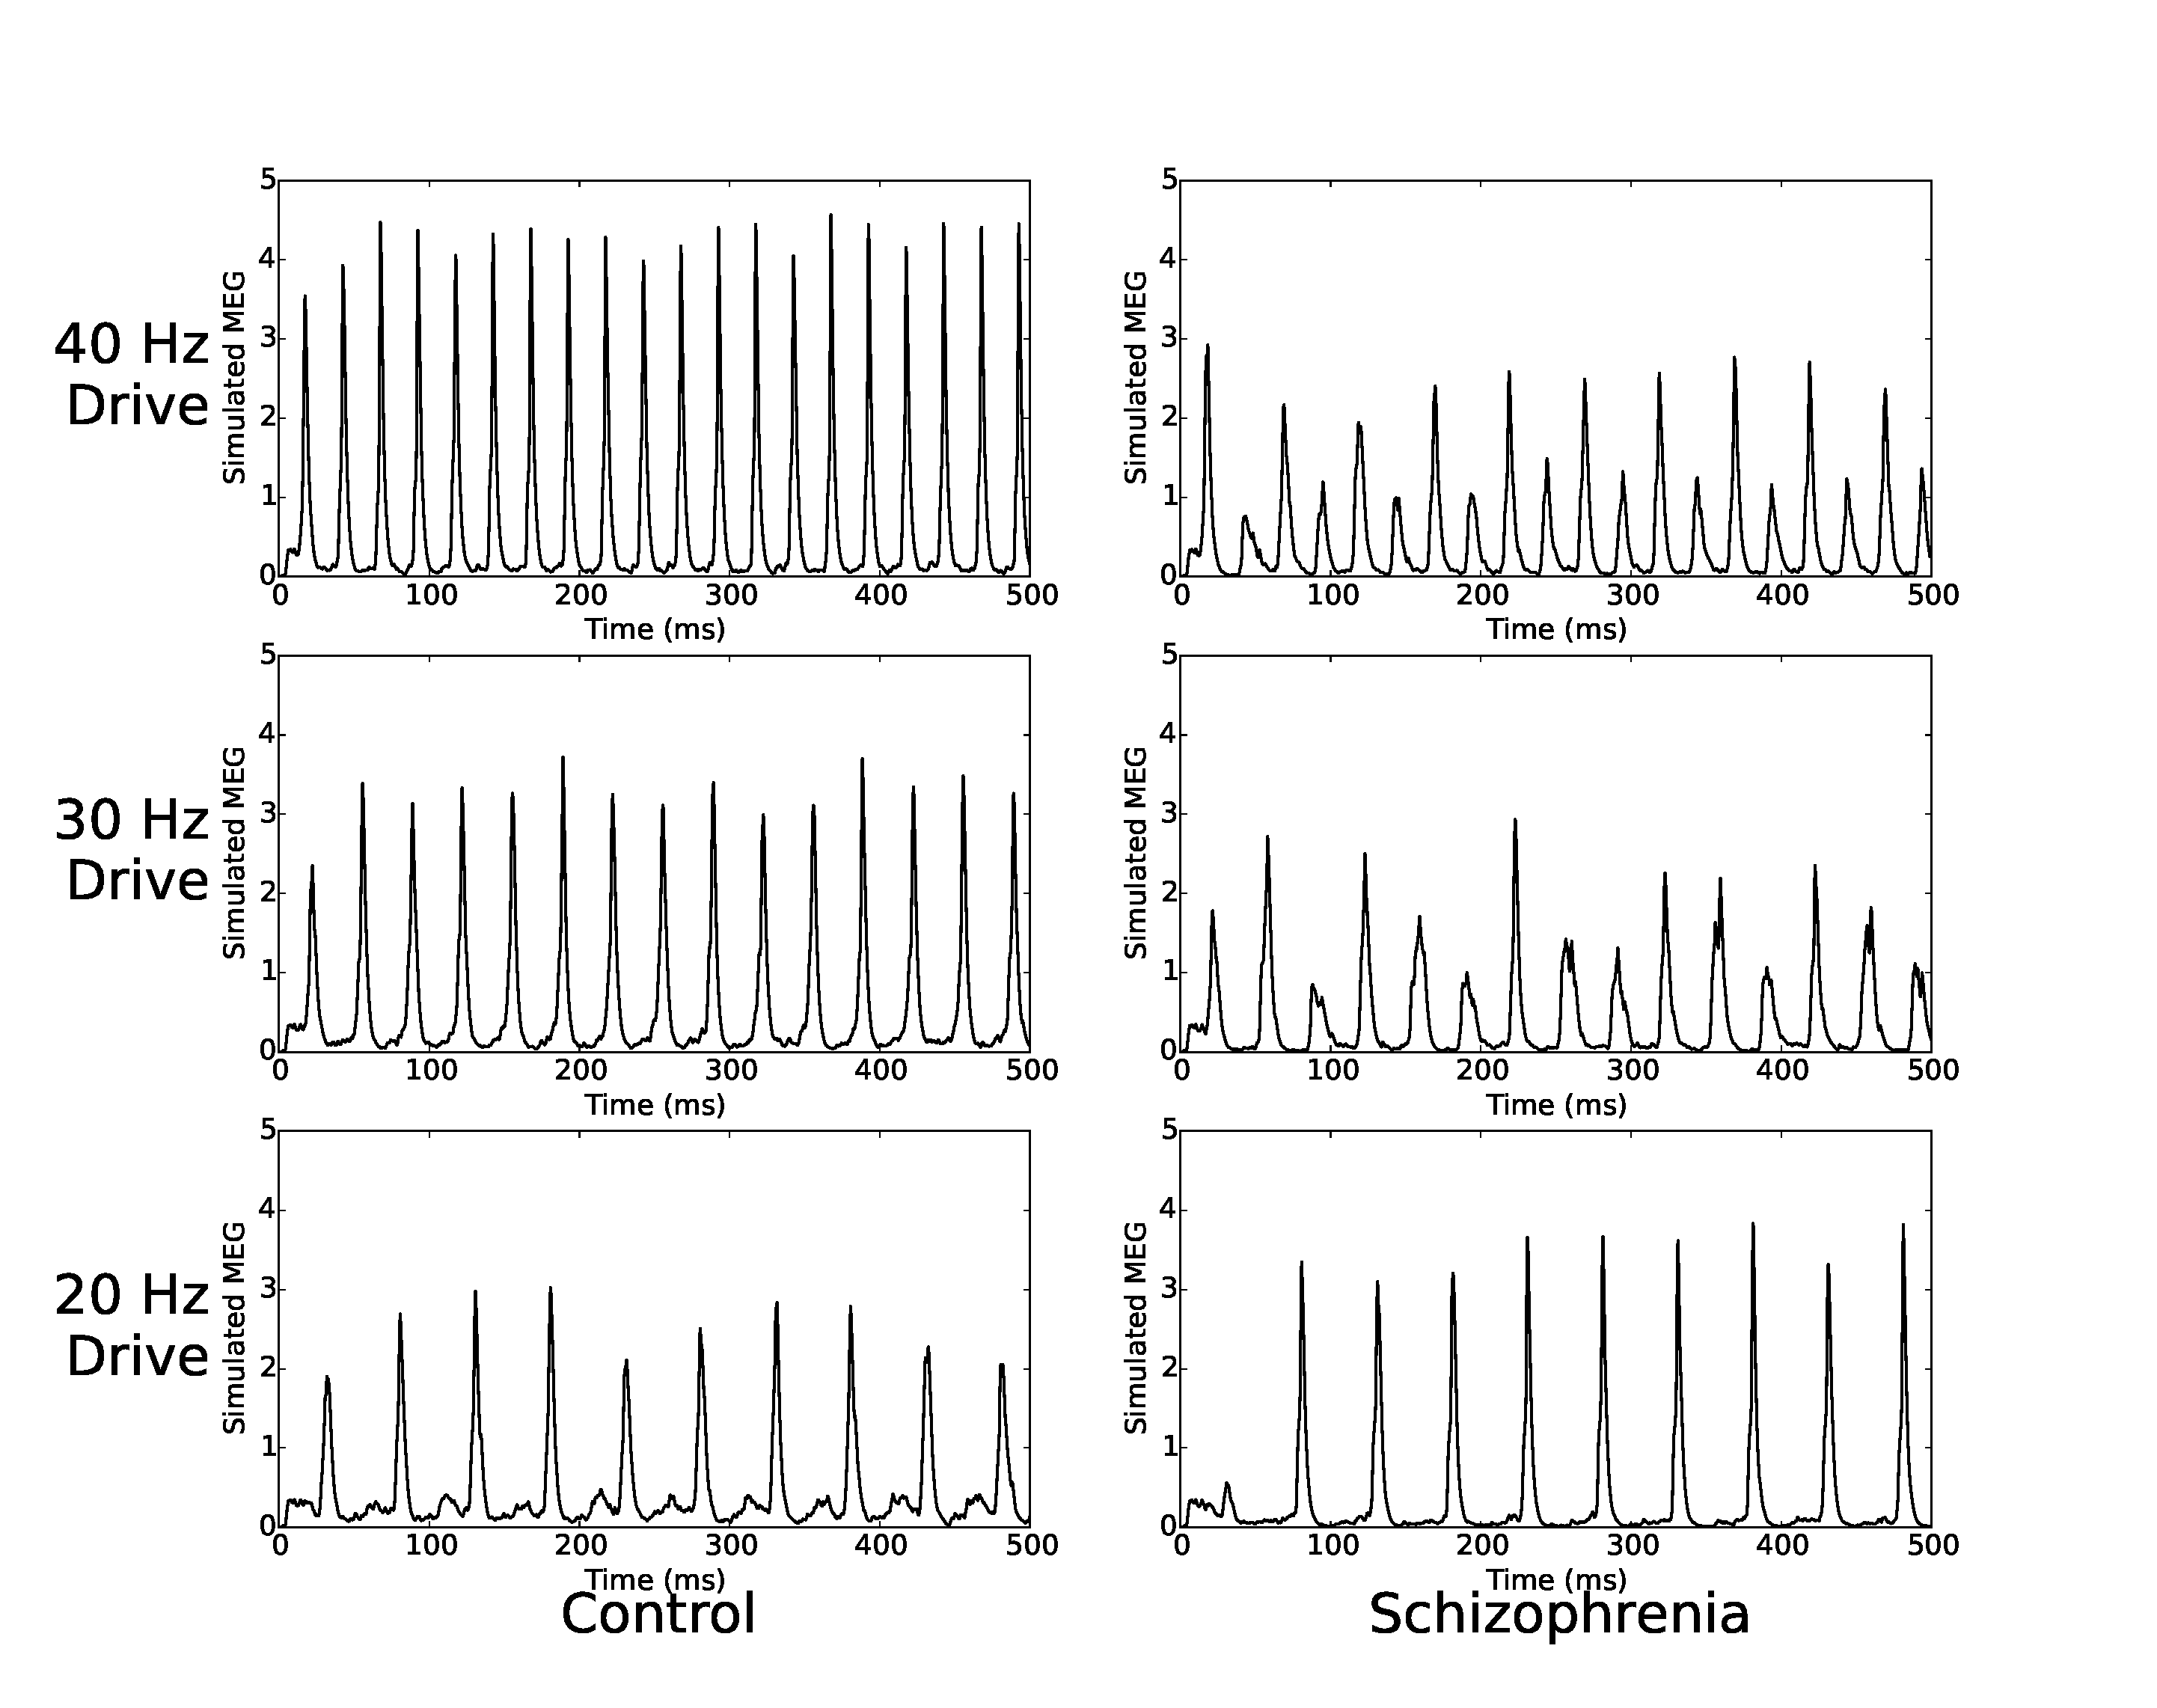
\includegraphics{Replication-Figure4.eps}
\caption{Replication of Figure 4: Raw simulated MEG signals (averaged
over 20 trials) for the control and the schizophrenic network at the
three different driving frequencies.}\label{fig:Vierling4}
\end{figure}

\begin{figure}
\centering
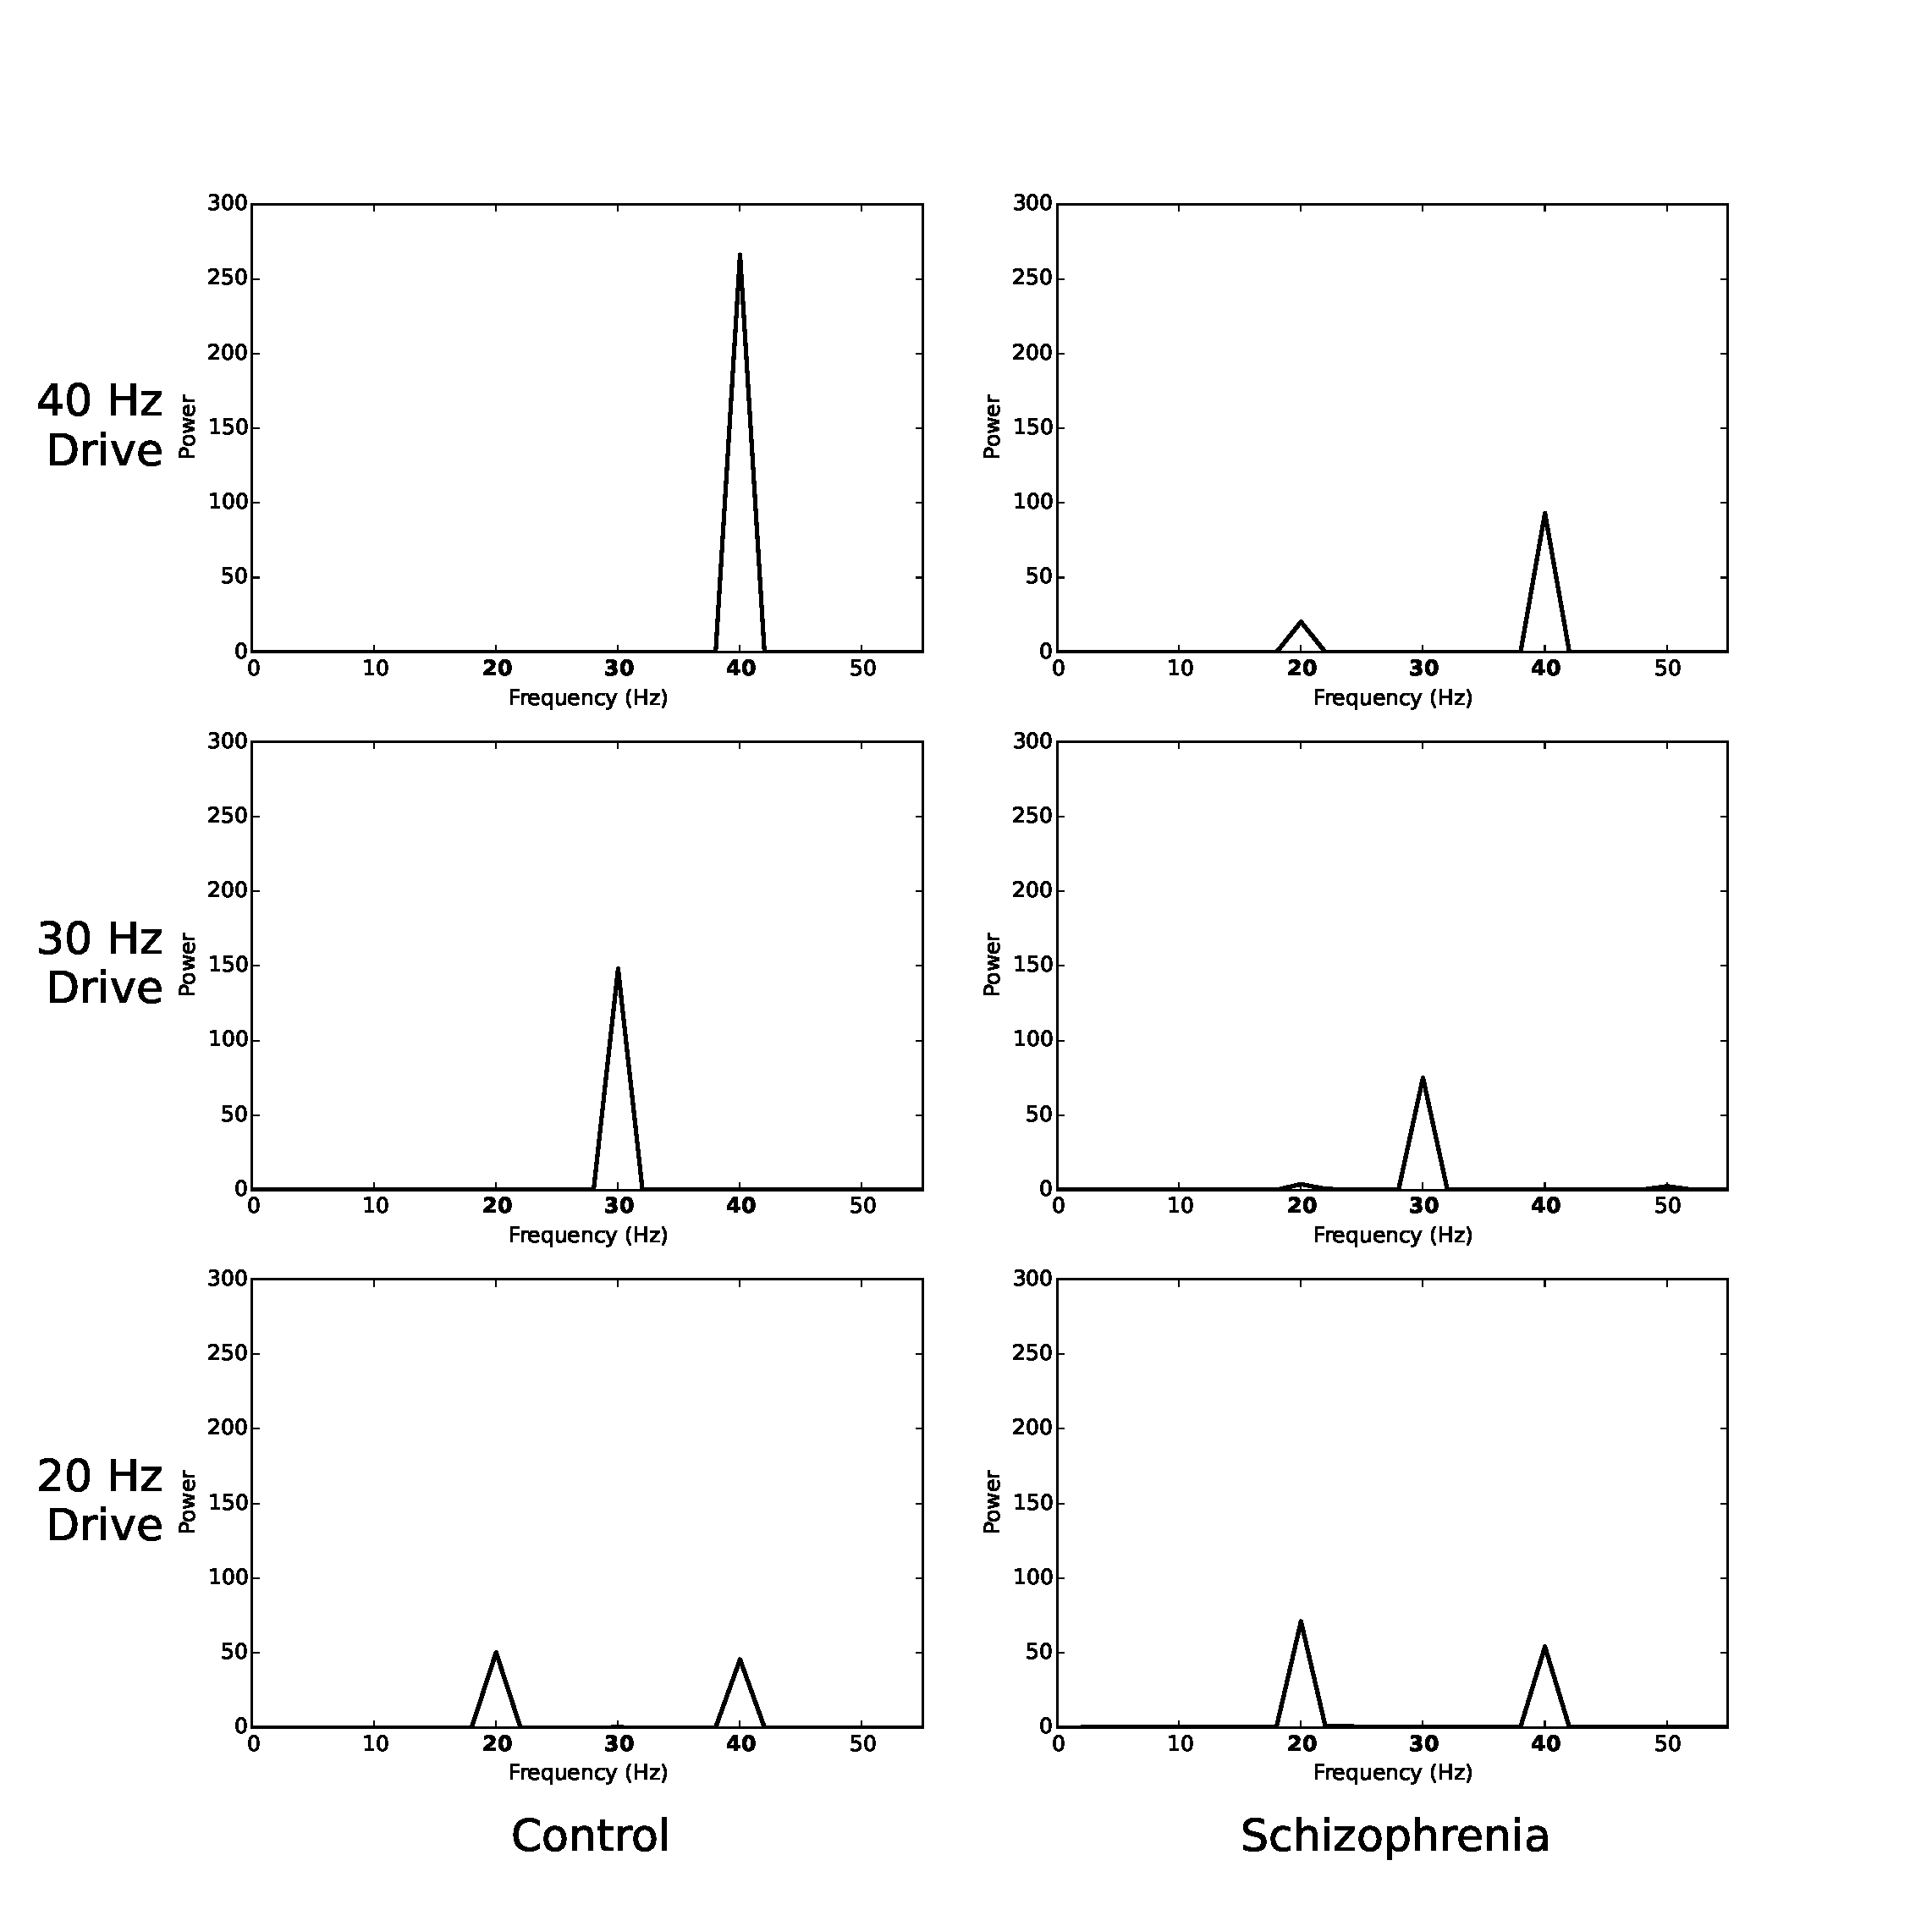
\includegraphics{Replication-Figure5.eps}
\caption{Replication of Figure 5: Power spectra of the averaged MEG
signals from \ref{fig:Vierling4}}\label{fig:Vierling5}
\end{figure}

After having looked at the model output averaged over 20 trials with
different noise, we also show single trial data which exemplify the main
model features , as was done in the original article. Figures
\ref{fig:Vierling6} and \ref{fig:Vierling7} show the model output in
response to 40 Hz drive input for the control and the schizophrenia
network, respectively. The strong entrainment in the control case, the
reduction of entrainment and the emergence of a subharmonic 20 Hz
component are again clearly visible. However, as before, in our model
implementation the emergent 20 Hz component is less pronounced than in
the original implementation (best seen in the excitatory population
activitydisplayed in the raster plot of \ref{fig:Vierling7}).

\begin{figure}
\centering
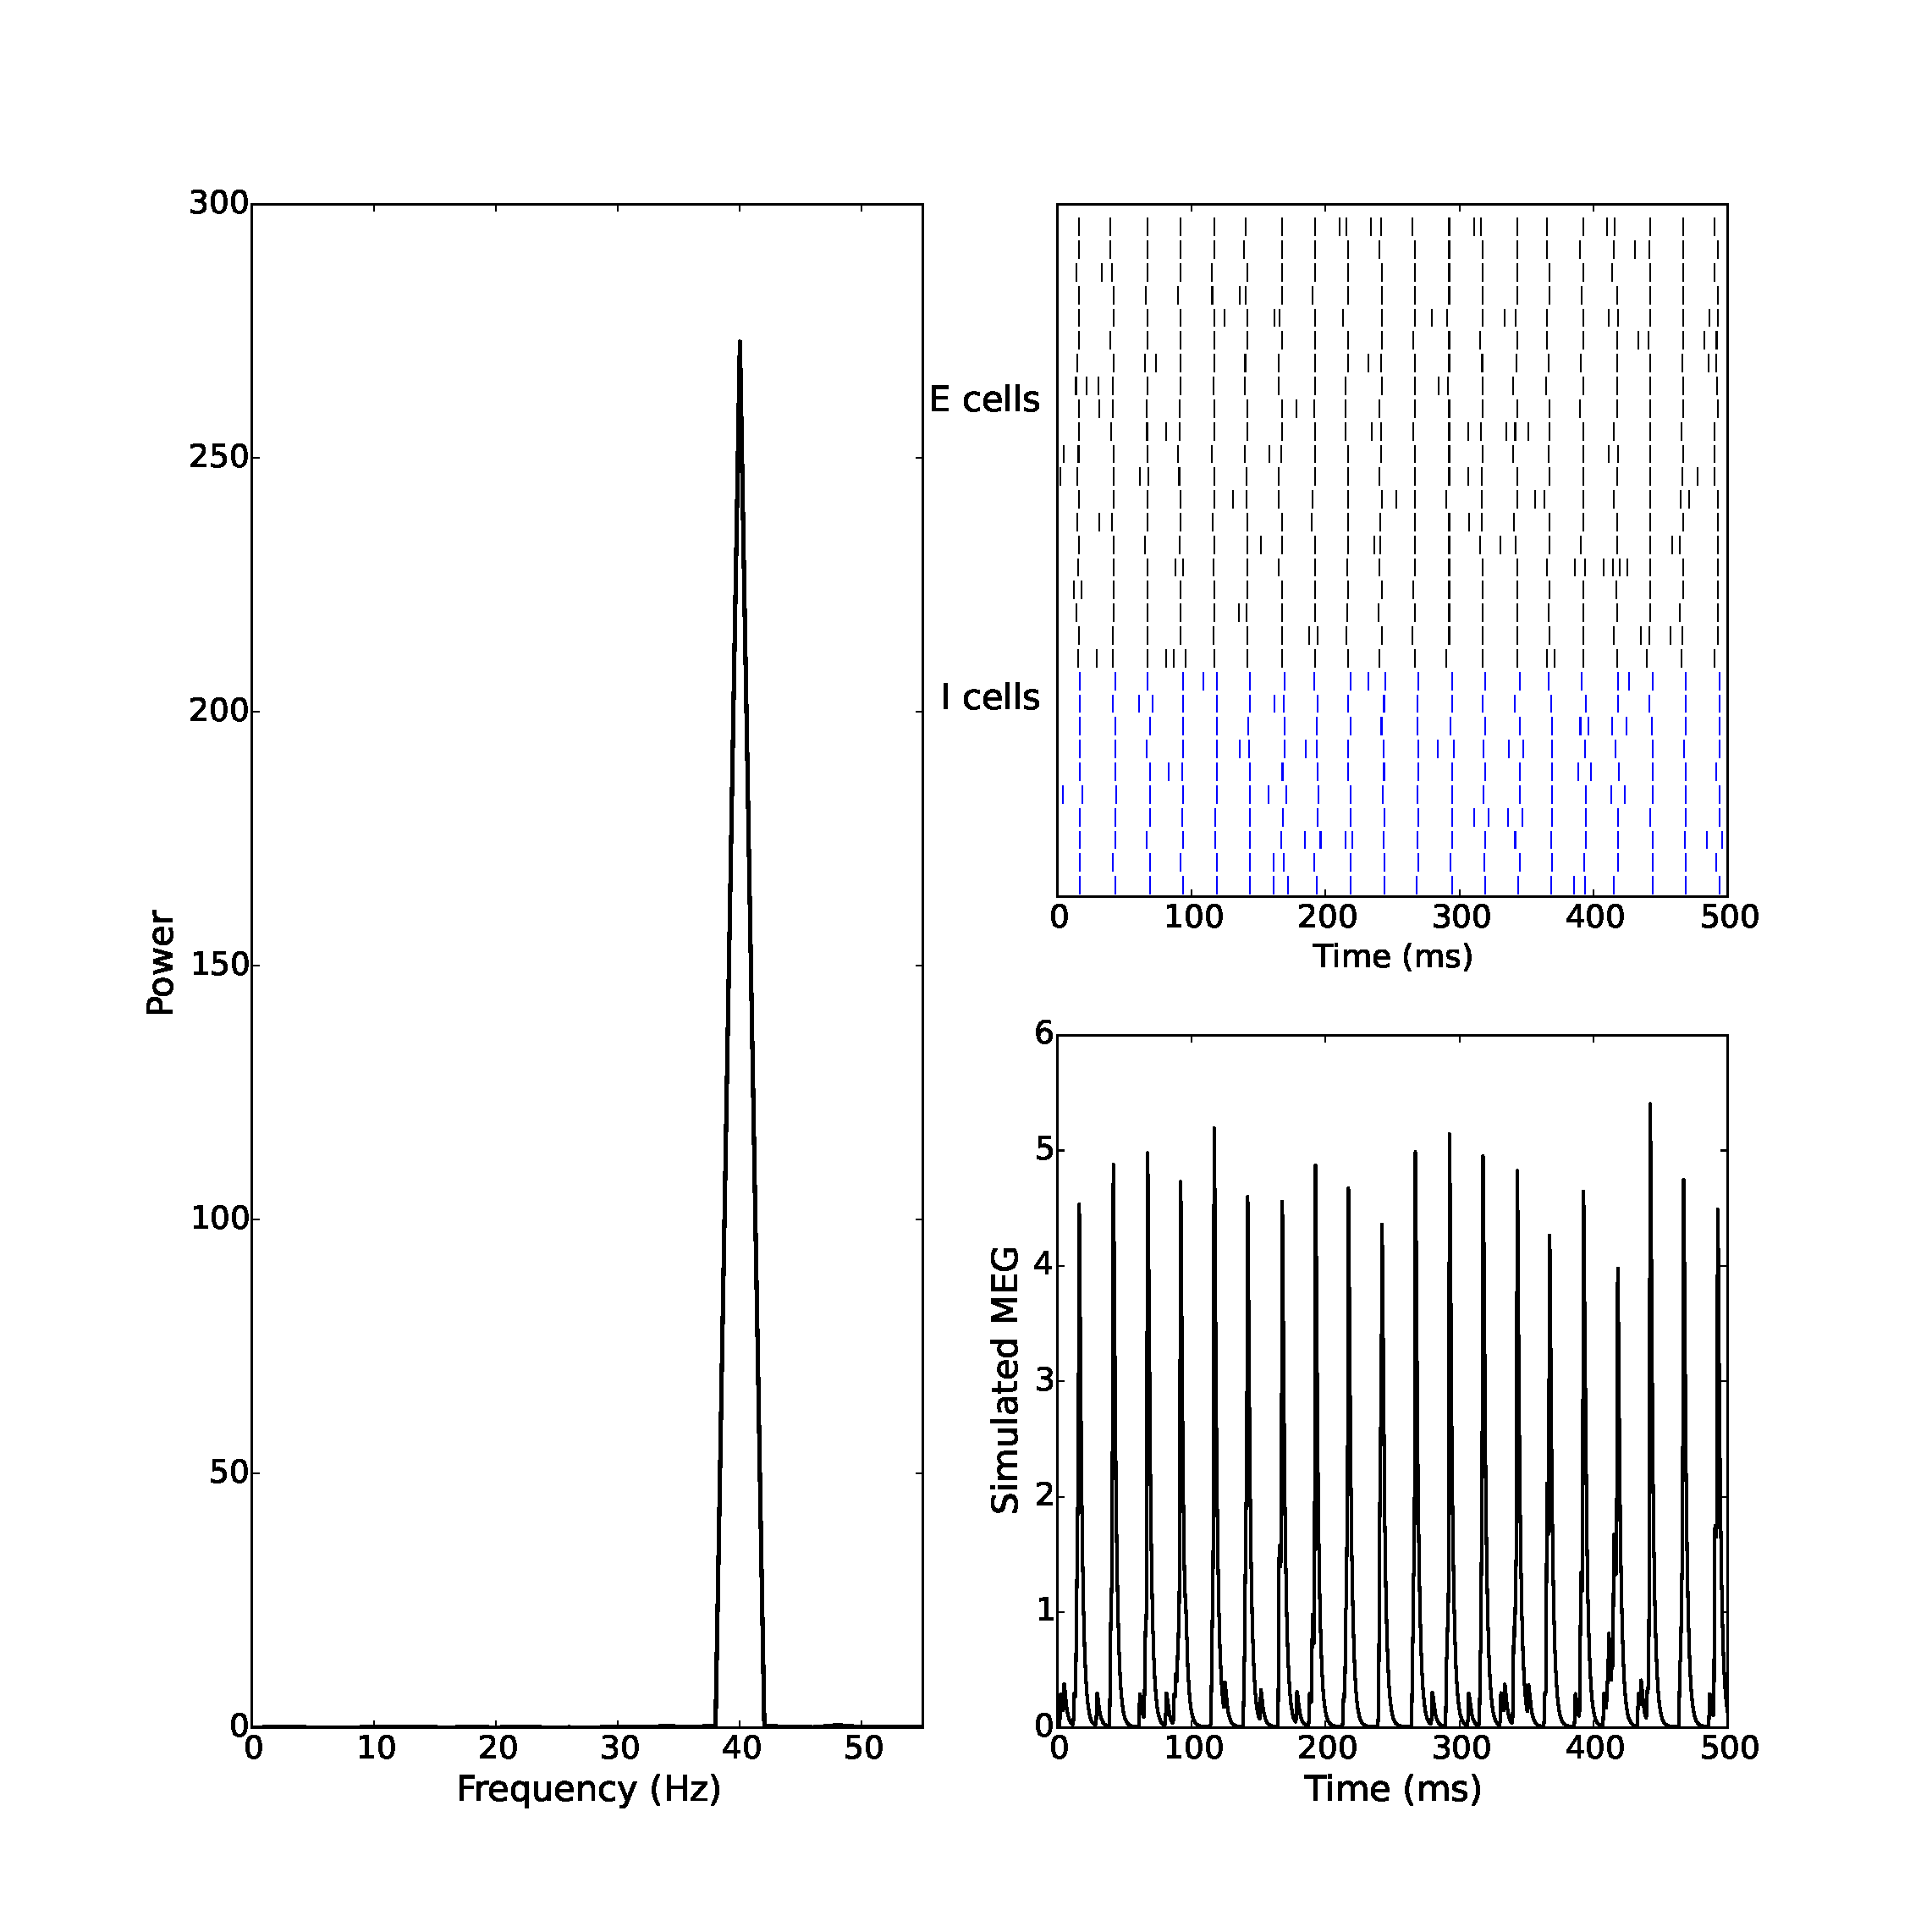
\includegraphics{Replication-Figure6.eps}
\caption{Replication of Figure 6: Single trial from the control network.
40 Hz drive. Network entrains to 40 Hz, as can be seen in the frequency
diagram, raster plot and MEG trace.}\label{fig:Vierling6}
\end{figure}

\begin{figure}
\centering
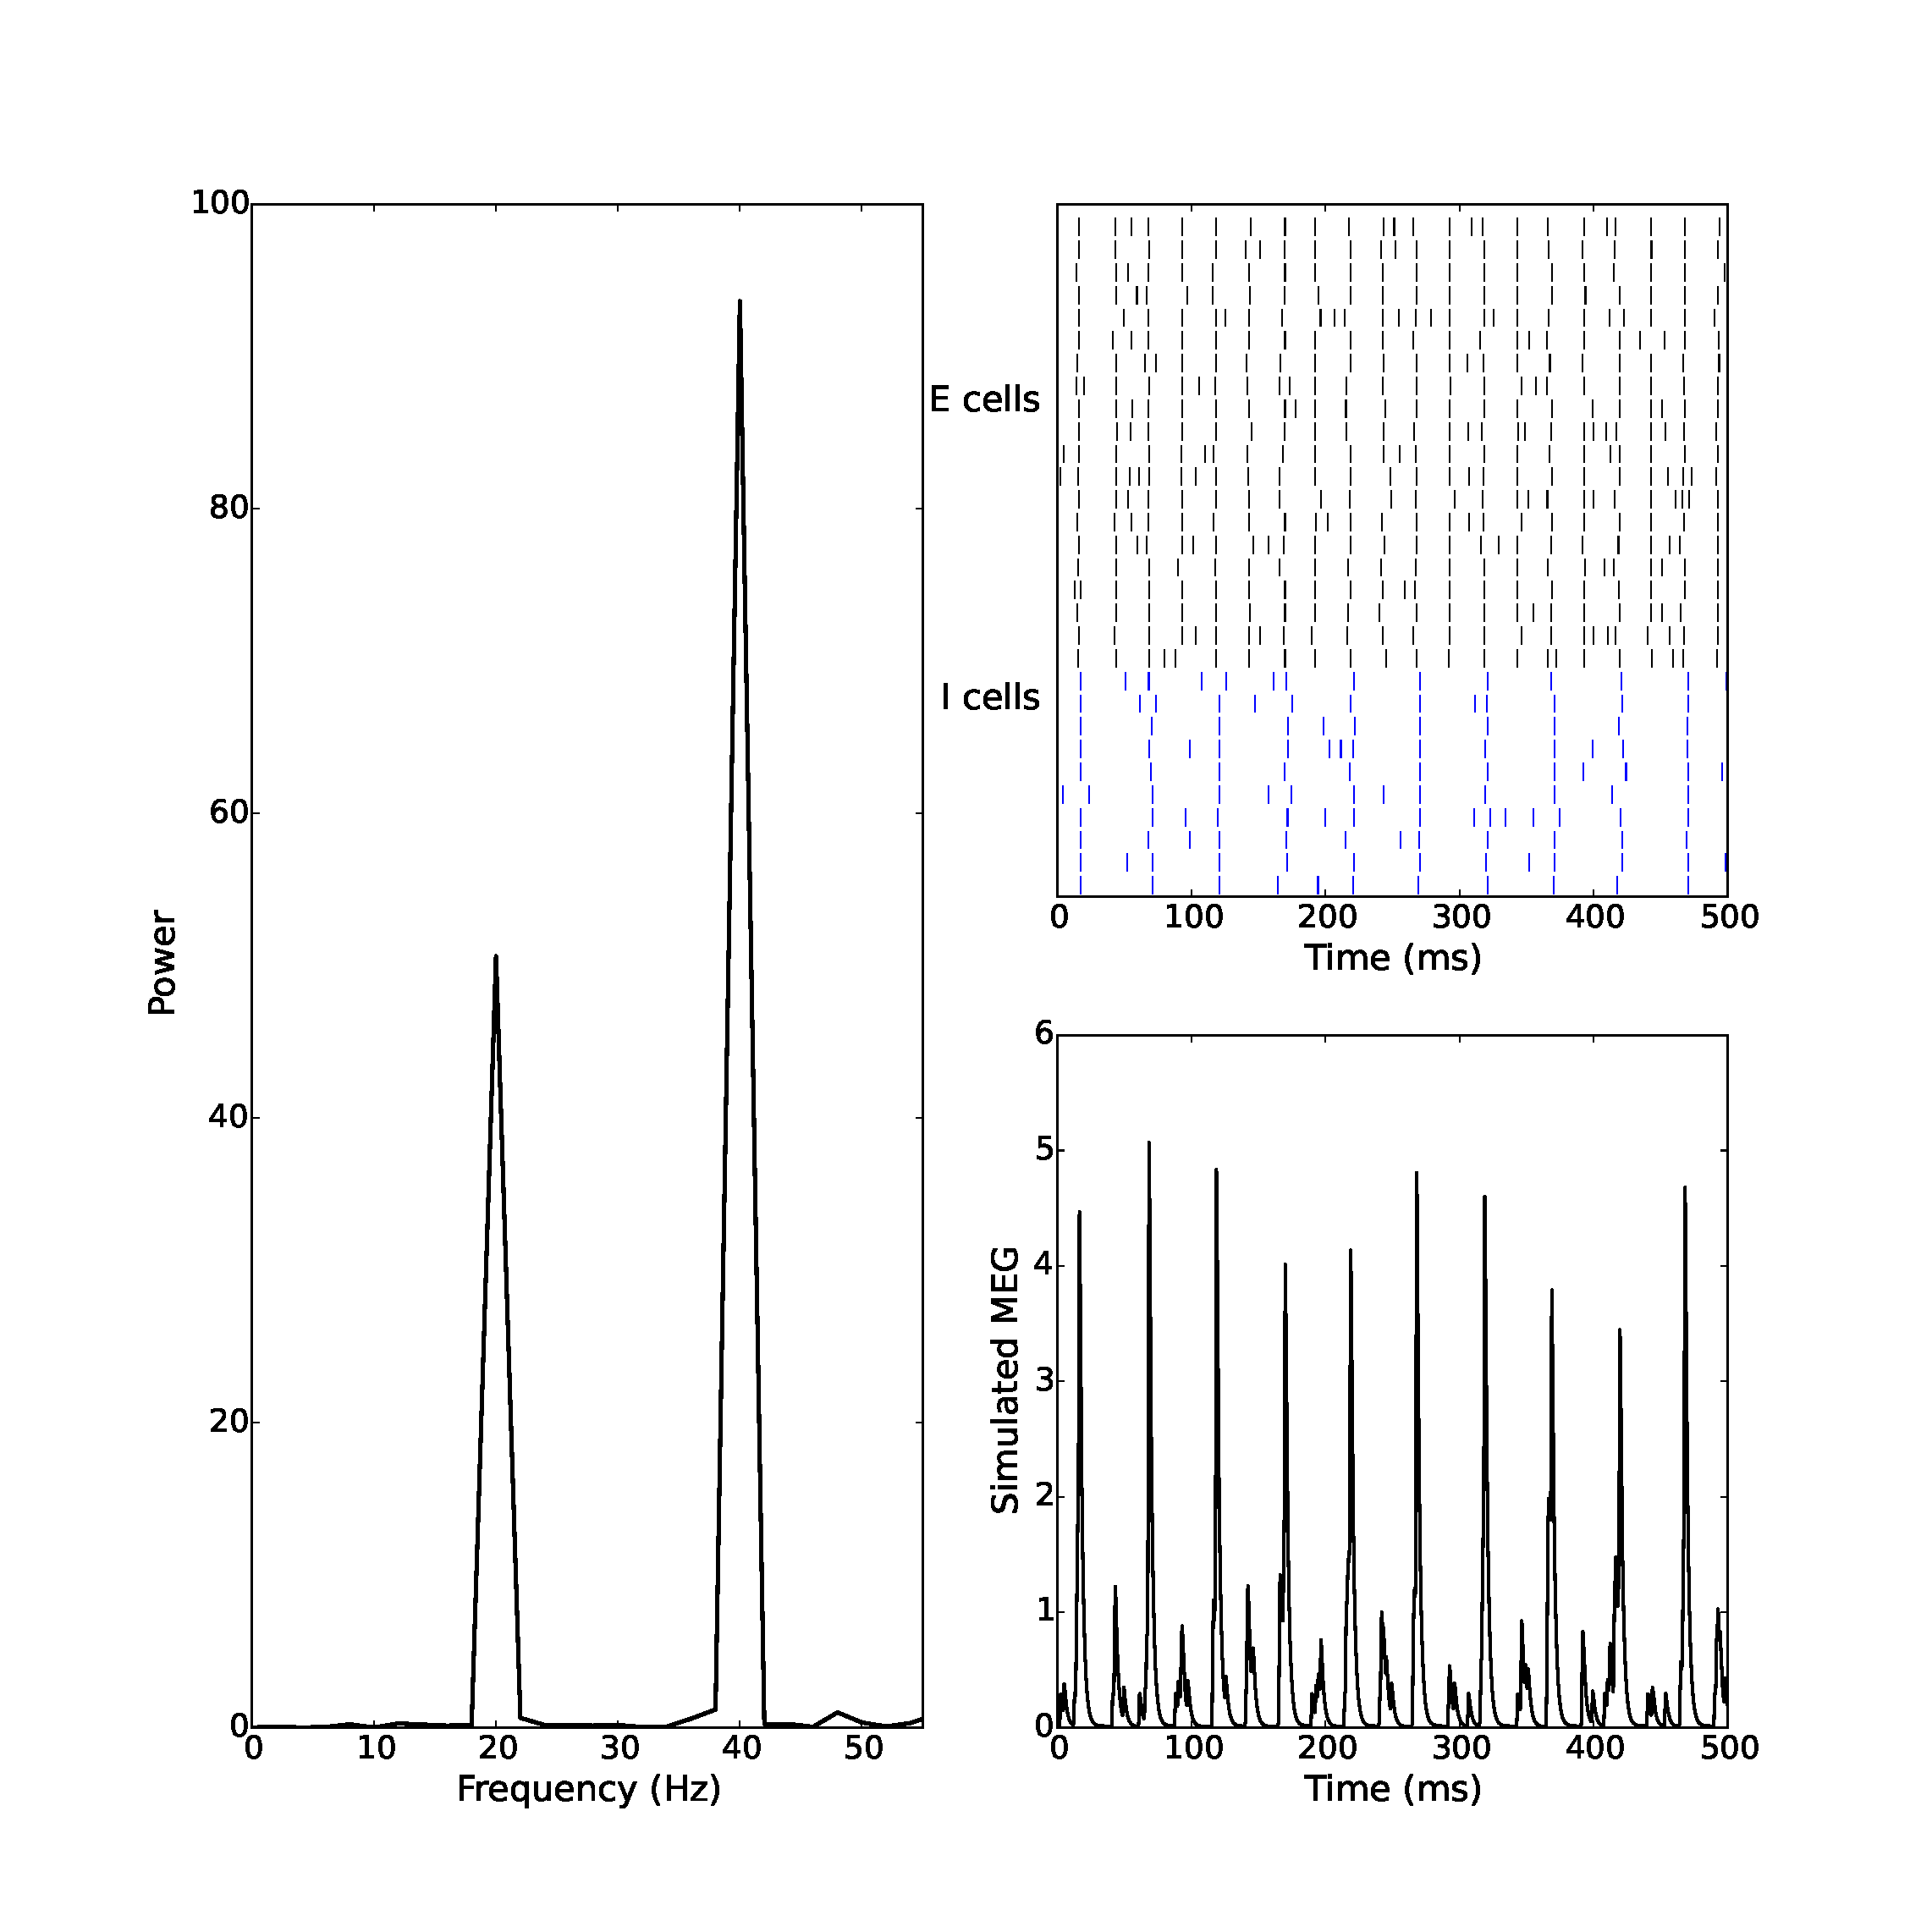
\includegraphics{Replication-Figure7.eps}
\caption{Replication of Figure 7: Single trial from the schizophrenia
network. 40 Hz drive. Network entrains to 40 Hz but also shows a strong
20 Hz component, as can be seen in the frequency diagram, raster plot
and MEG trace. Especially the inhibitory neurons only entrain to a 20 Hz
rhythm (see raster plot).}\label{fig:Vierling7}
\end{figure}

Figures \ref{fig:Vierling10} and \ref{fig:Vierling11} show the
model output in response to 20 Hz drive for the control and the
schizophrenia network, respectively. Again, main features of the
original model are faithfully reproduced.

\begin{figure}
\centering
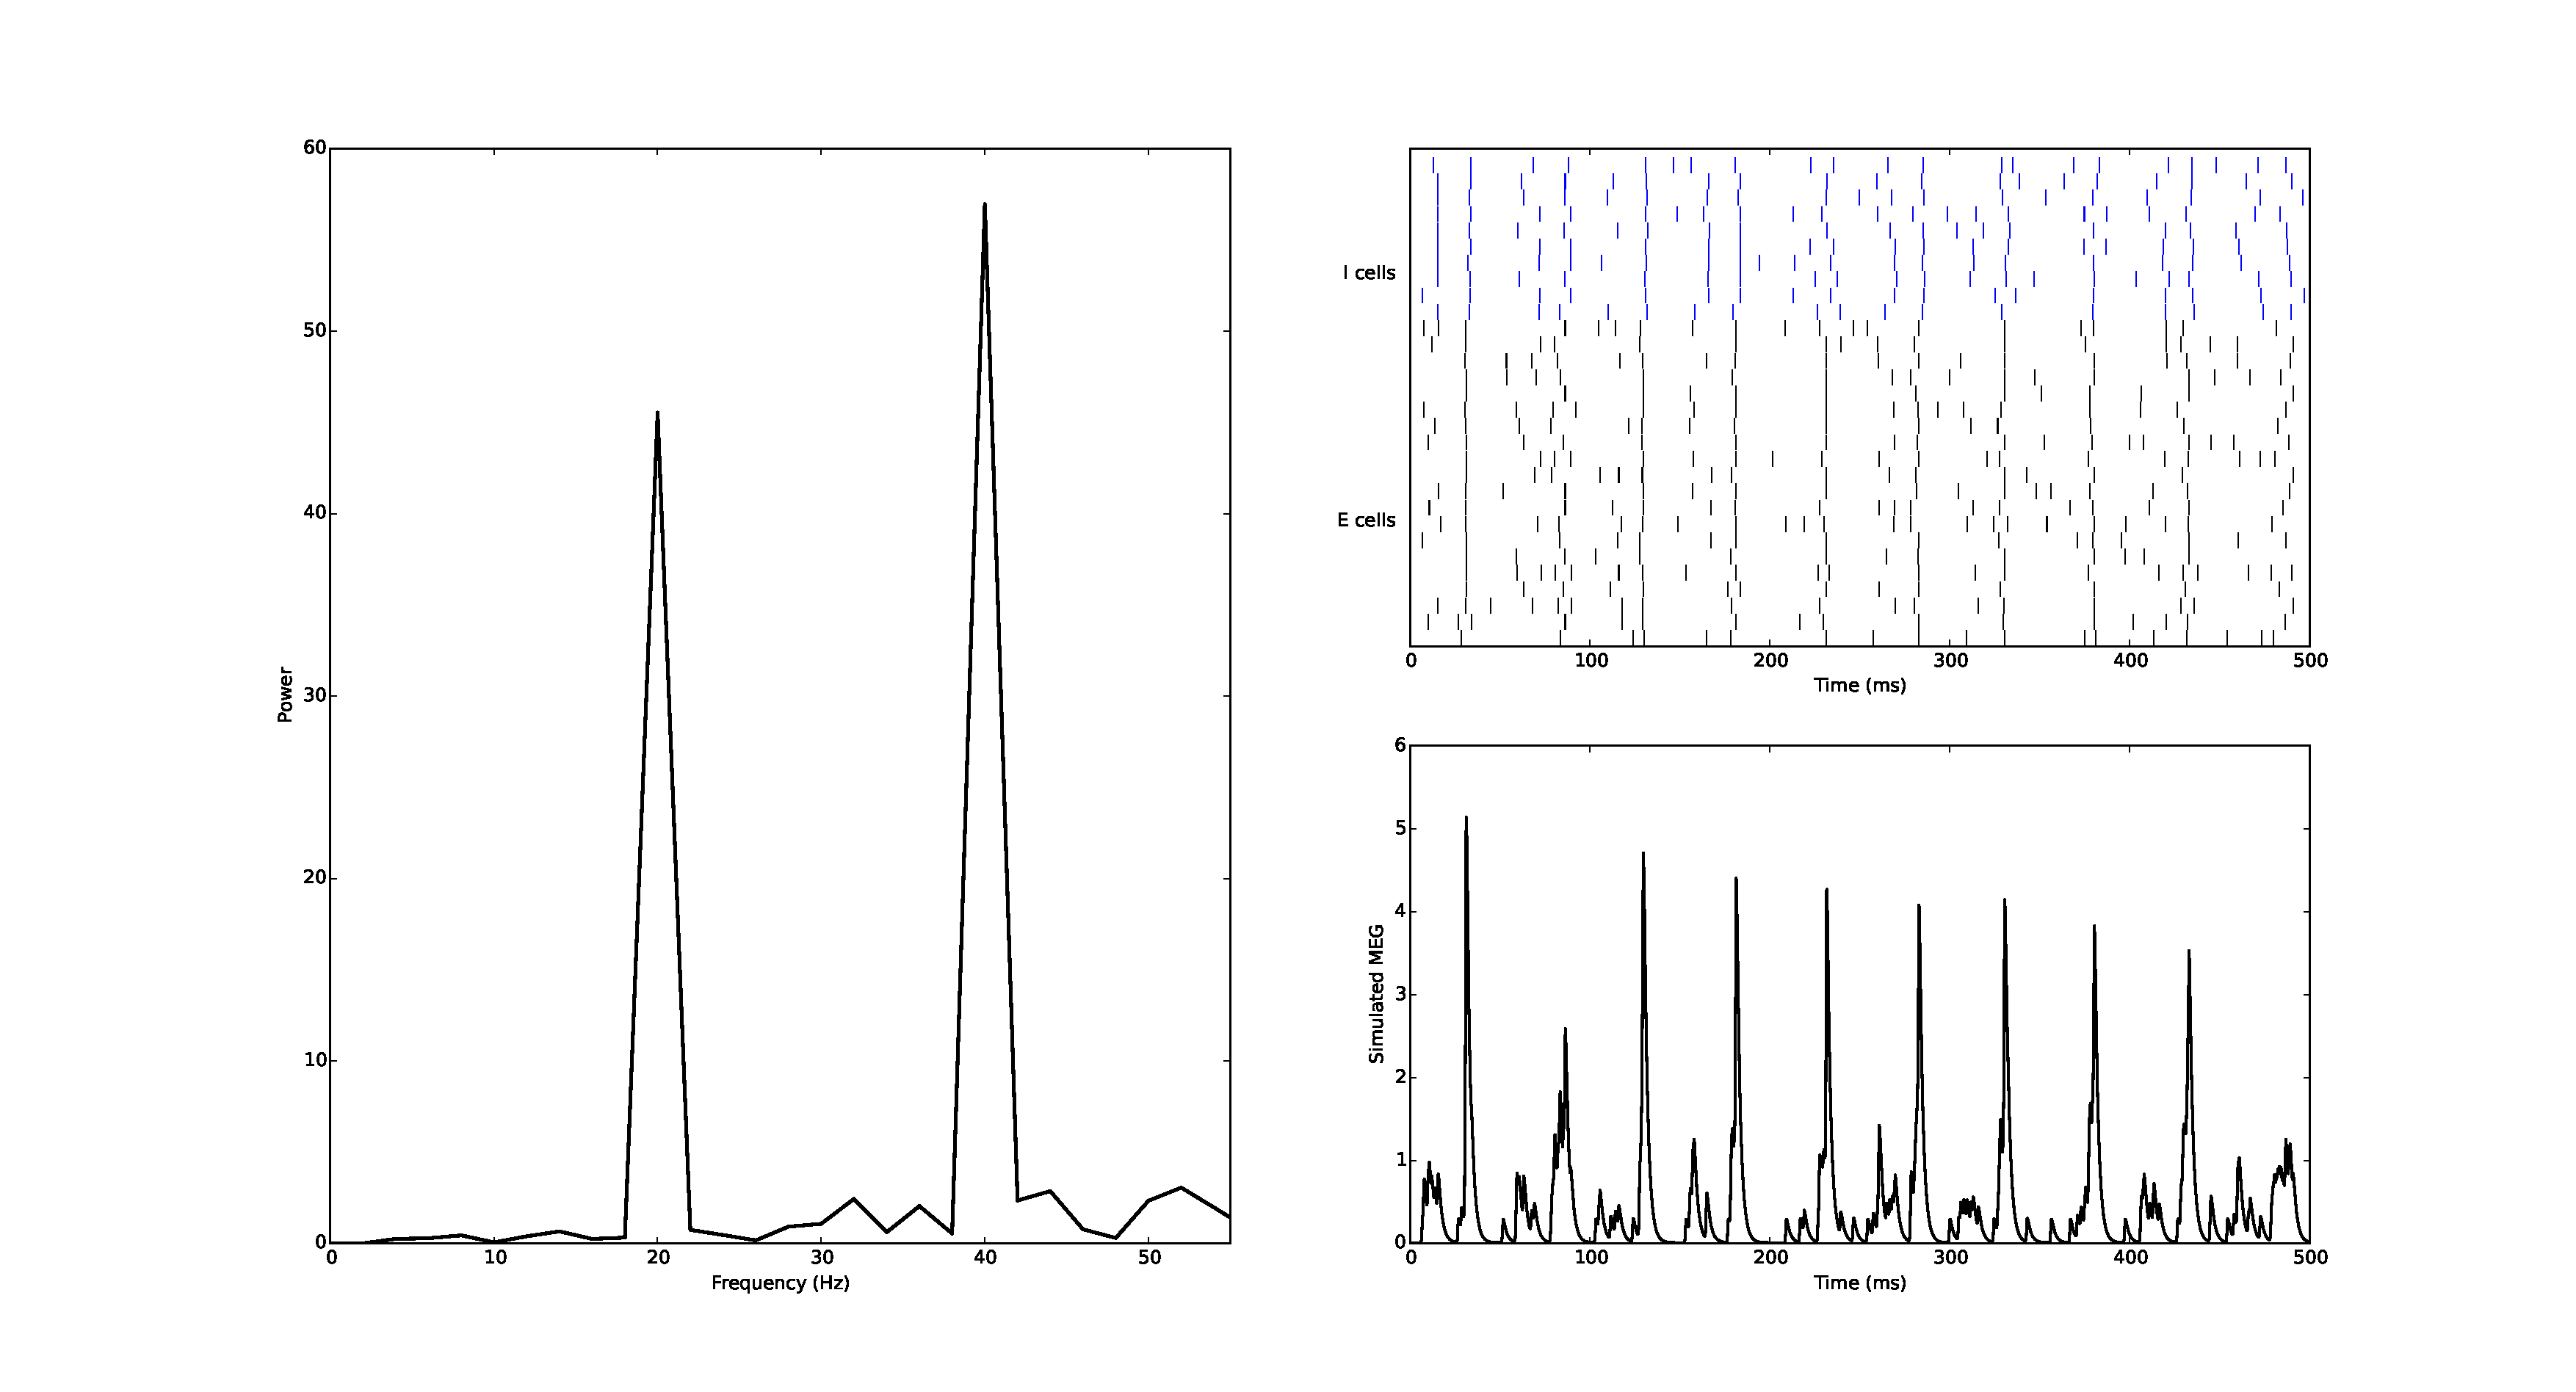
\includegraphics{Replication-Figure10.eps}
\caption{Replication of Figure 10: Single trial from the control
network. 20 Hz drive. Network entrains to 20 Hz but also shows a 40 Hz
component, as can be seen in the frequency diagram, raster plot and MEG
trace.}\label{fig:Vierling10}
\end{figure}

\begin{figure}
\centering
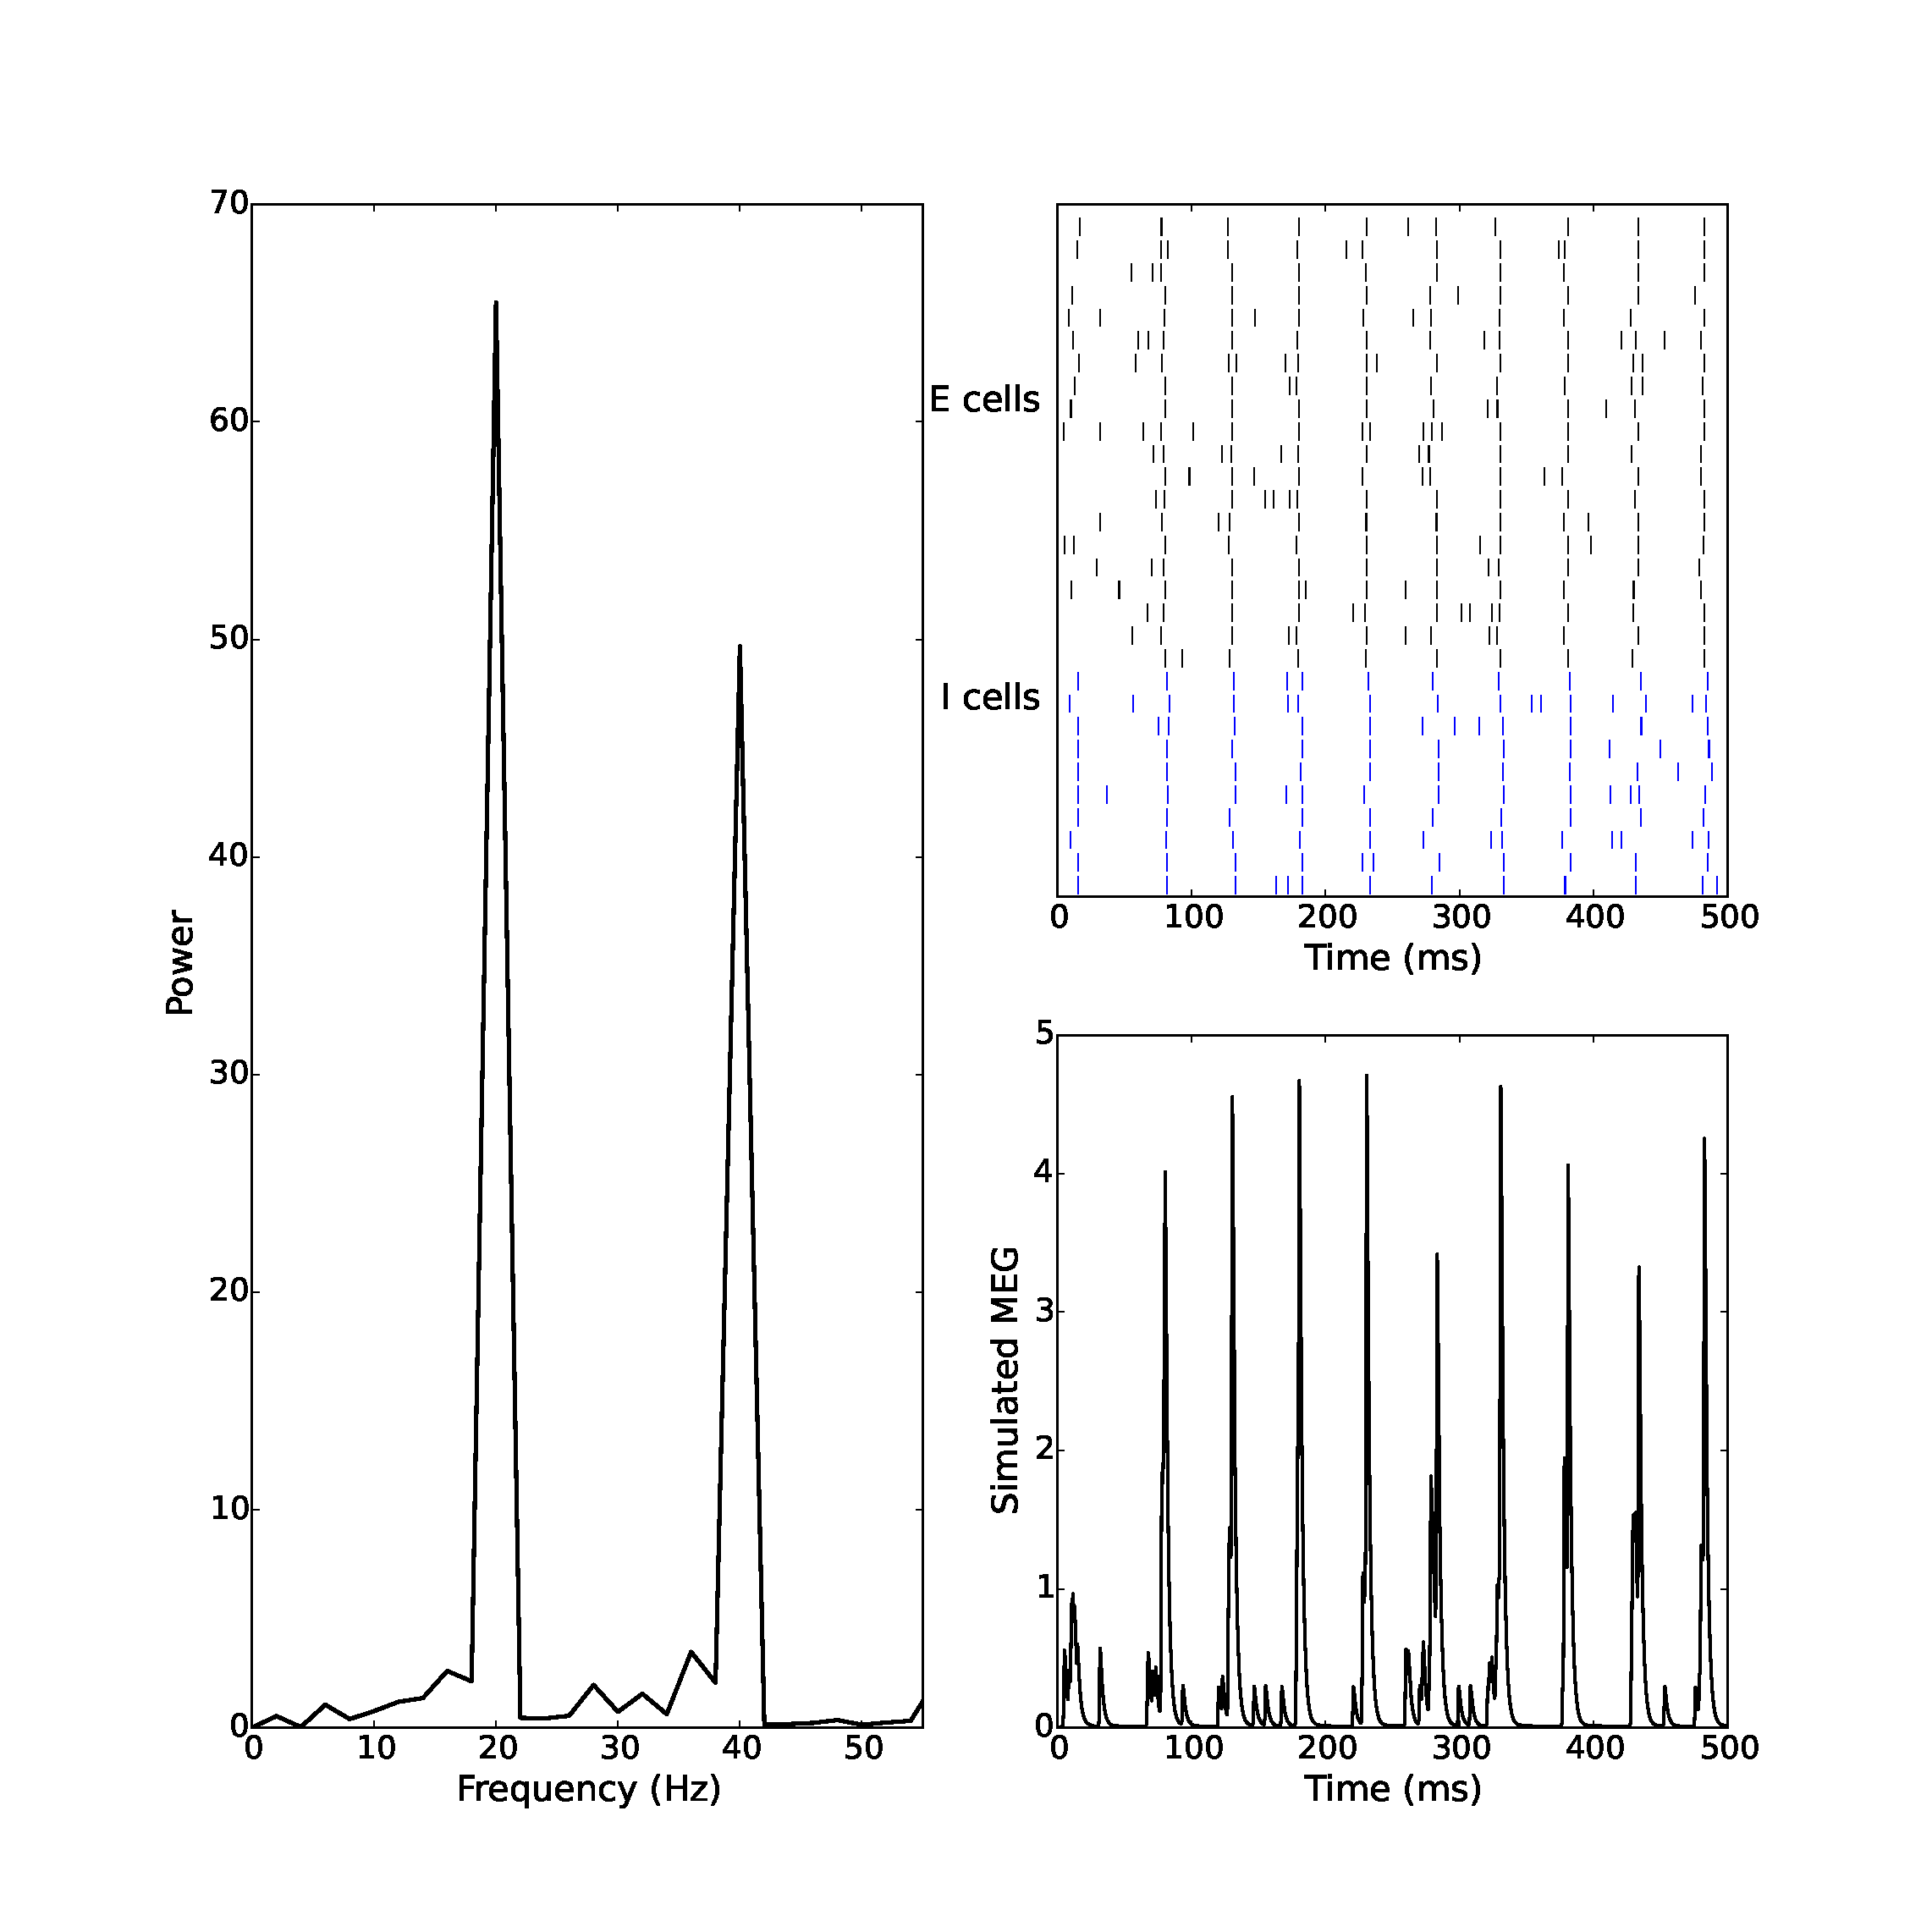
\includegraphics{Replication-Figure11.eps}
\caption{Replication of Figure 11: Single trial from the schizophrenia
network. 20 Hz drive. Network entrains to 20 Hz without 40 Hz component,
as can be seen in the frequency diagram, raster plot and MEG trace. note
that the 40 Hz power in the power spectrum is a
harmonic.}\label{fig:Vierling11}
\end{figure}



\subsection{Exploration of the Discrepancies between Original and Reimplementation}
In this section we explore possible scenarios that might explain the less pronounced main features in the reimplementation.

We explore the influence of the background noise. The main mechanism behind the emergence of a 20 Hz component in response
to 40 Hz drive in the schizophrenia network is the prolonged inhibition which suppresses activity in every second 40 Hz cycle. In the absence
of noise the network responds with a pure 20 Hz oscillation (see Figures \ref{fig:NoiseExplorationMEG} left upper panel and \ref{fig:NoiseExplorationPSD} left upper panel). However, the background noise
gives sufficient input to some excitatory cells to overcome this suppression and also fire in between the 20 Hz cycles. This results in a mixed response, 
where power is split between 20 Hz and 40 Hz. The ratio of this split depends on the strength of the noise. Therefore, we asked whether the less pronounced
20 Hz component in our reimplementation might simply come from a too high background noise amplitude. Figures \ref{fig:NoiseExplorationMEG} (left middle and lower panels  and \ref{fig:NoiseExplorationPSD} left middle and lower panels, show the 
response (MEG signal and power spectral density, respectivey) to a 40 Hz drive in the cases, where we scaled down the noise to 75\% and 50\%, respectively. It can clearly be seen that the 20 Hz component increases, when
the noise strength decreases. However, as can be seen in right panels, showing the response of the control network to 20 Hz drive,
is that downscaling of the background noise reduces the 40 Hz component in response to 20 Hz drive. This is not surprising since background noise drives excitatory cells to fire in between 20 Hz cycles in the control network, resulting
in the 40 Hz component. This component is suppressed in the schizophrenia network due to the prolonged inhibition.
Summarising, a difference in the strength of the background noise might be an explanation for the discrepancy between original and reimplementation. However, only a reduction of noise solely for the schizophrenia network 
fully replicates the original results. 

\begin{figure}
\centering
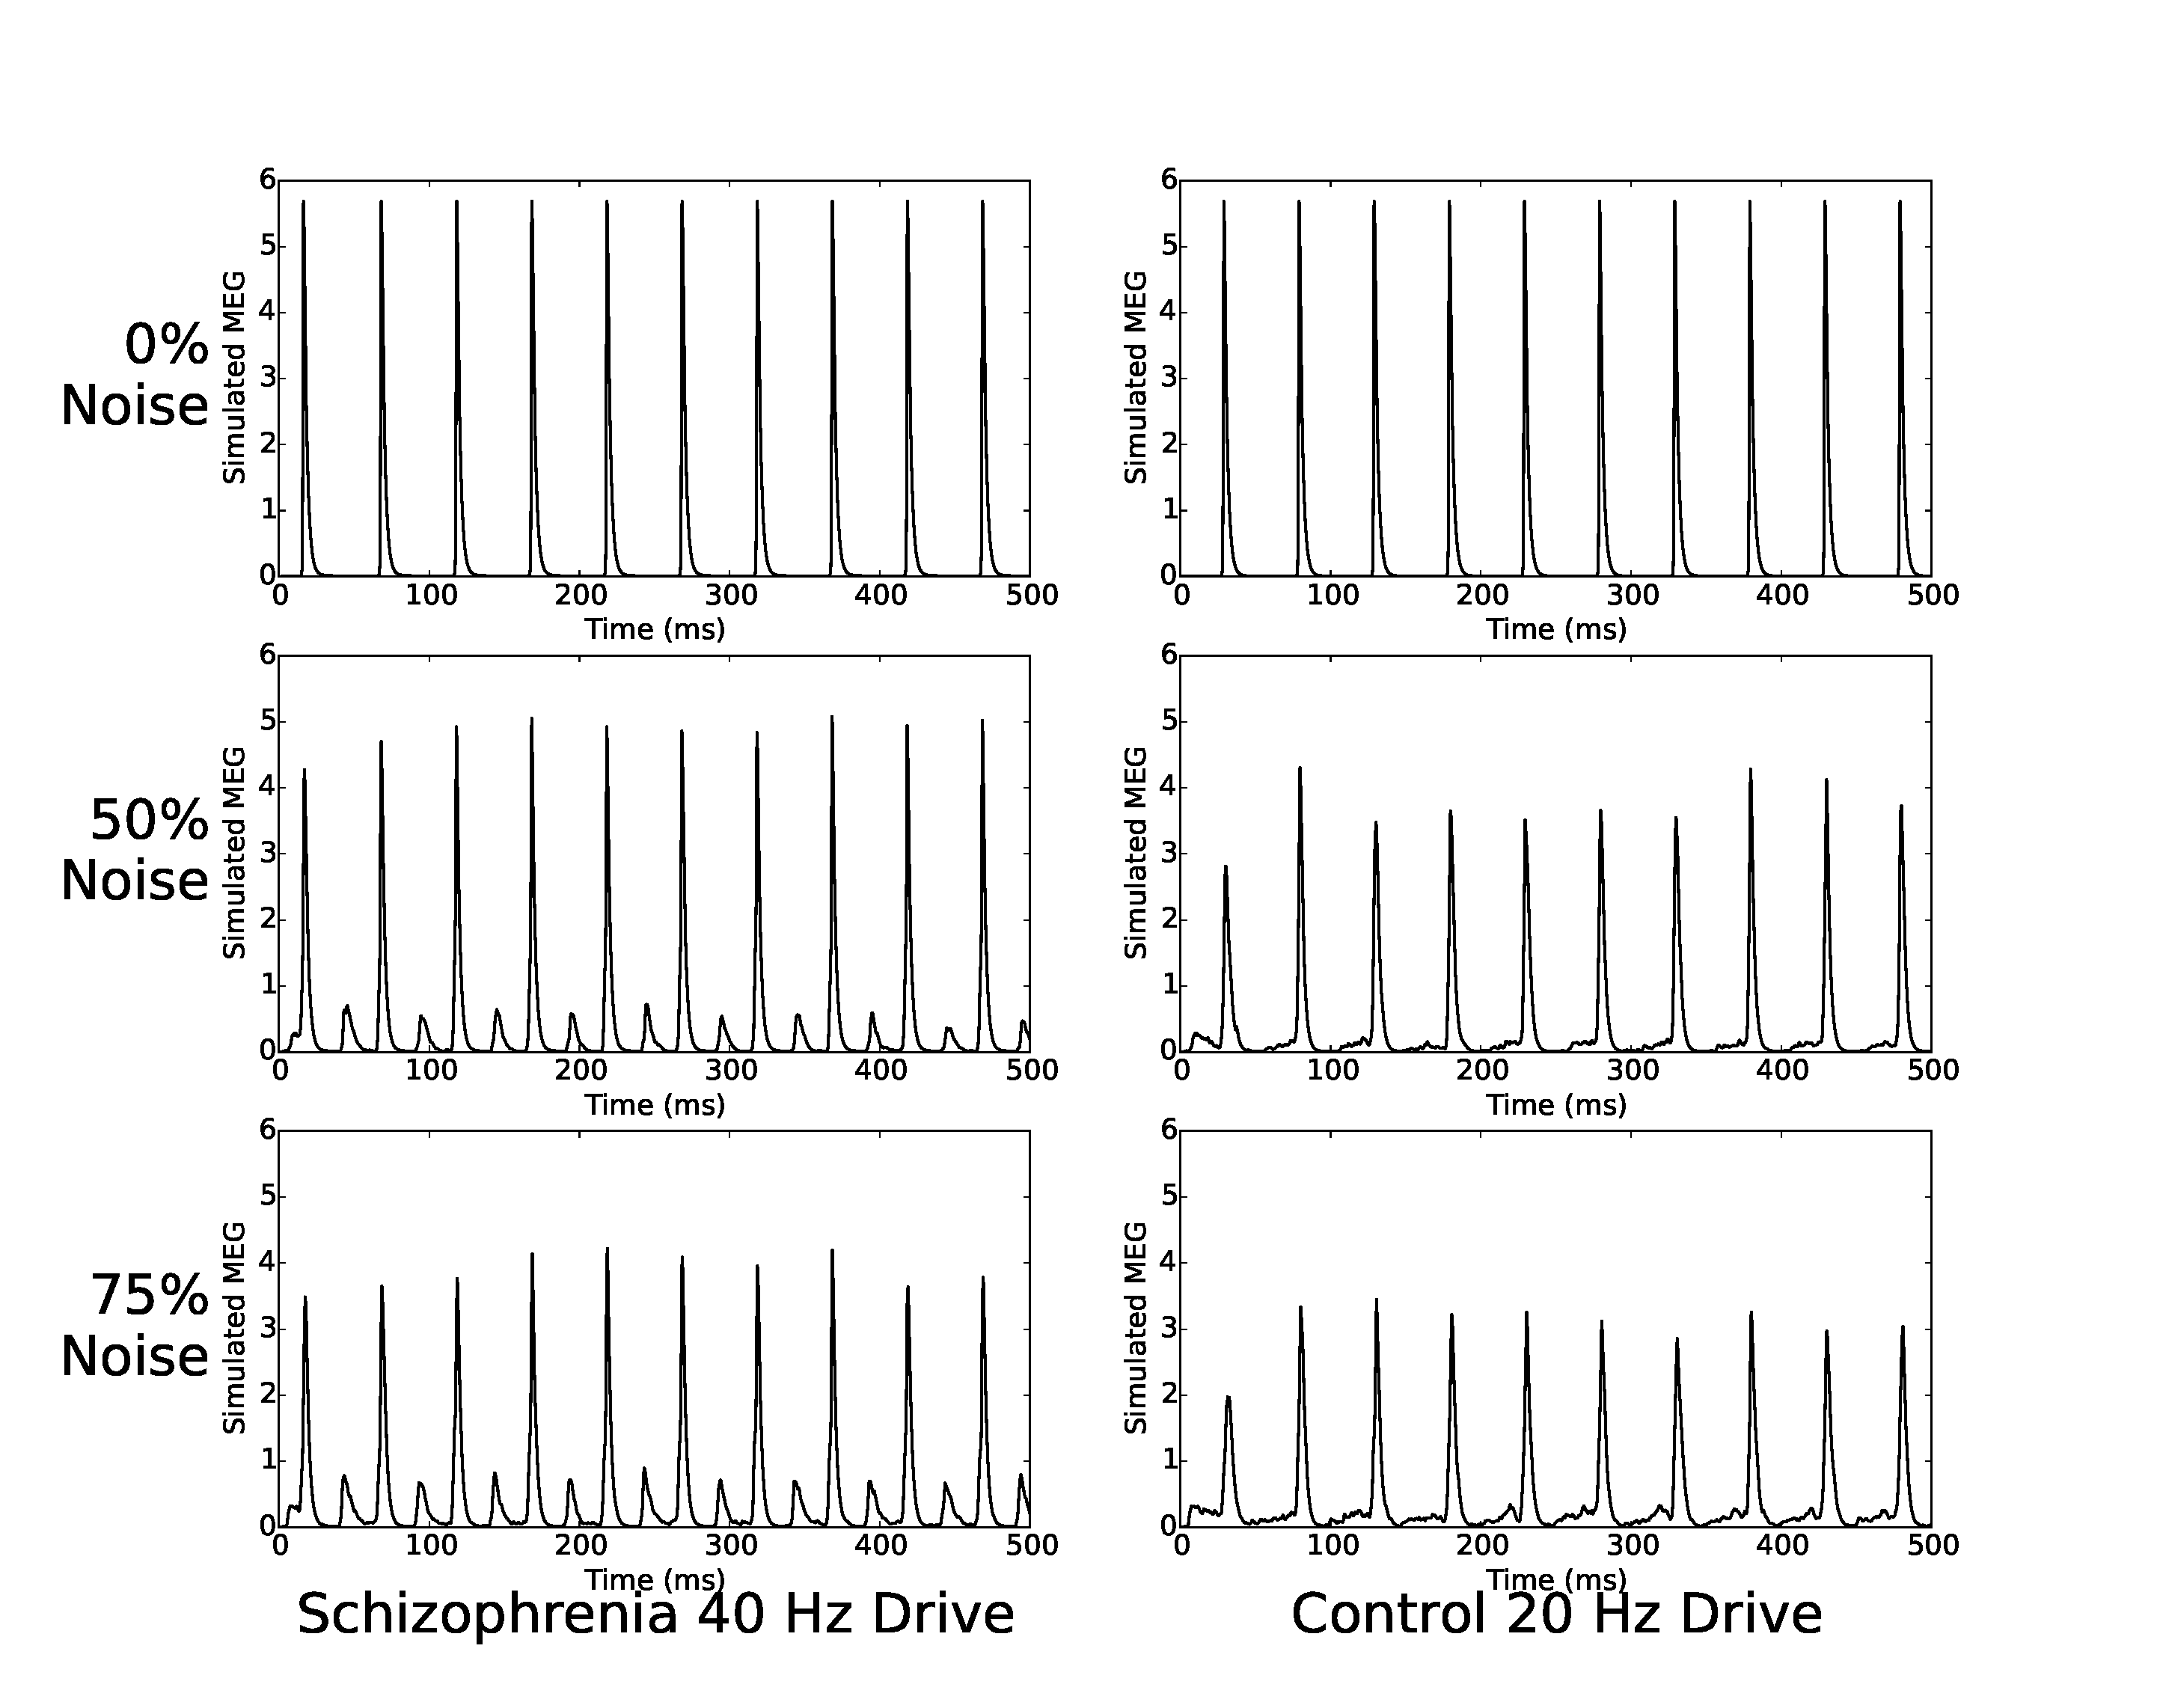
\includegraphics{Noise-Exploration-MEG.eps}
\caption{Replication of Figure 11: Single trial from the schizophrenia
network. 20 Hz drive. Network entrains to 20 Hz without 40 Hz component,
as can be seen in the frequency diagram, raster plot and MEG trace. note
that the 40 Hz power in the power spectrum is a
harmonic.}\label{fig:NoiseExplorationMEG}
\end{figure}

\begin{figure}
\centering
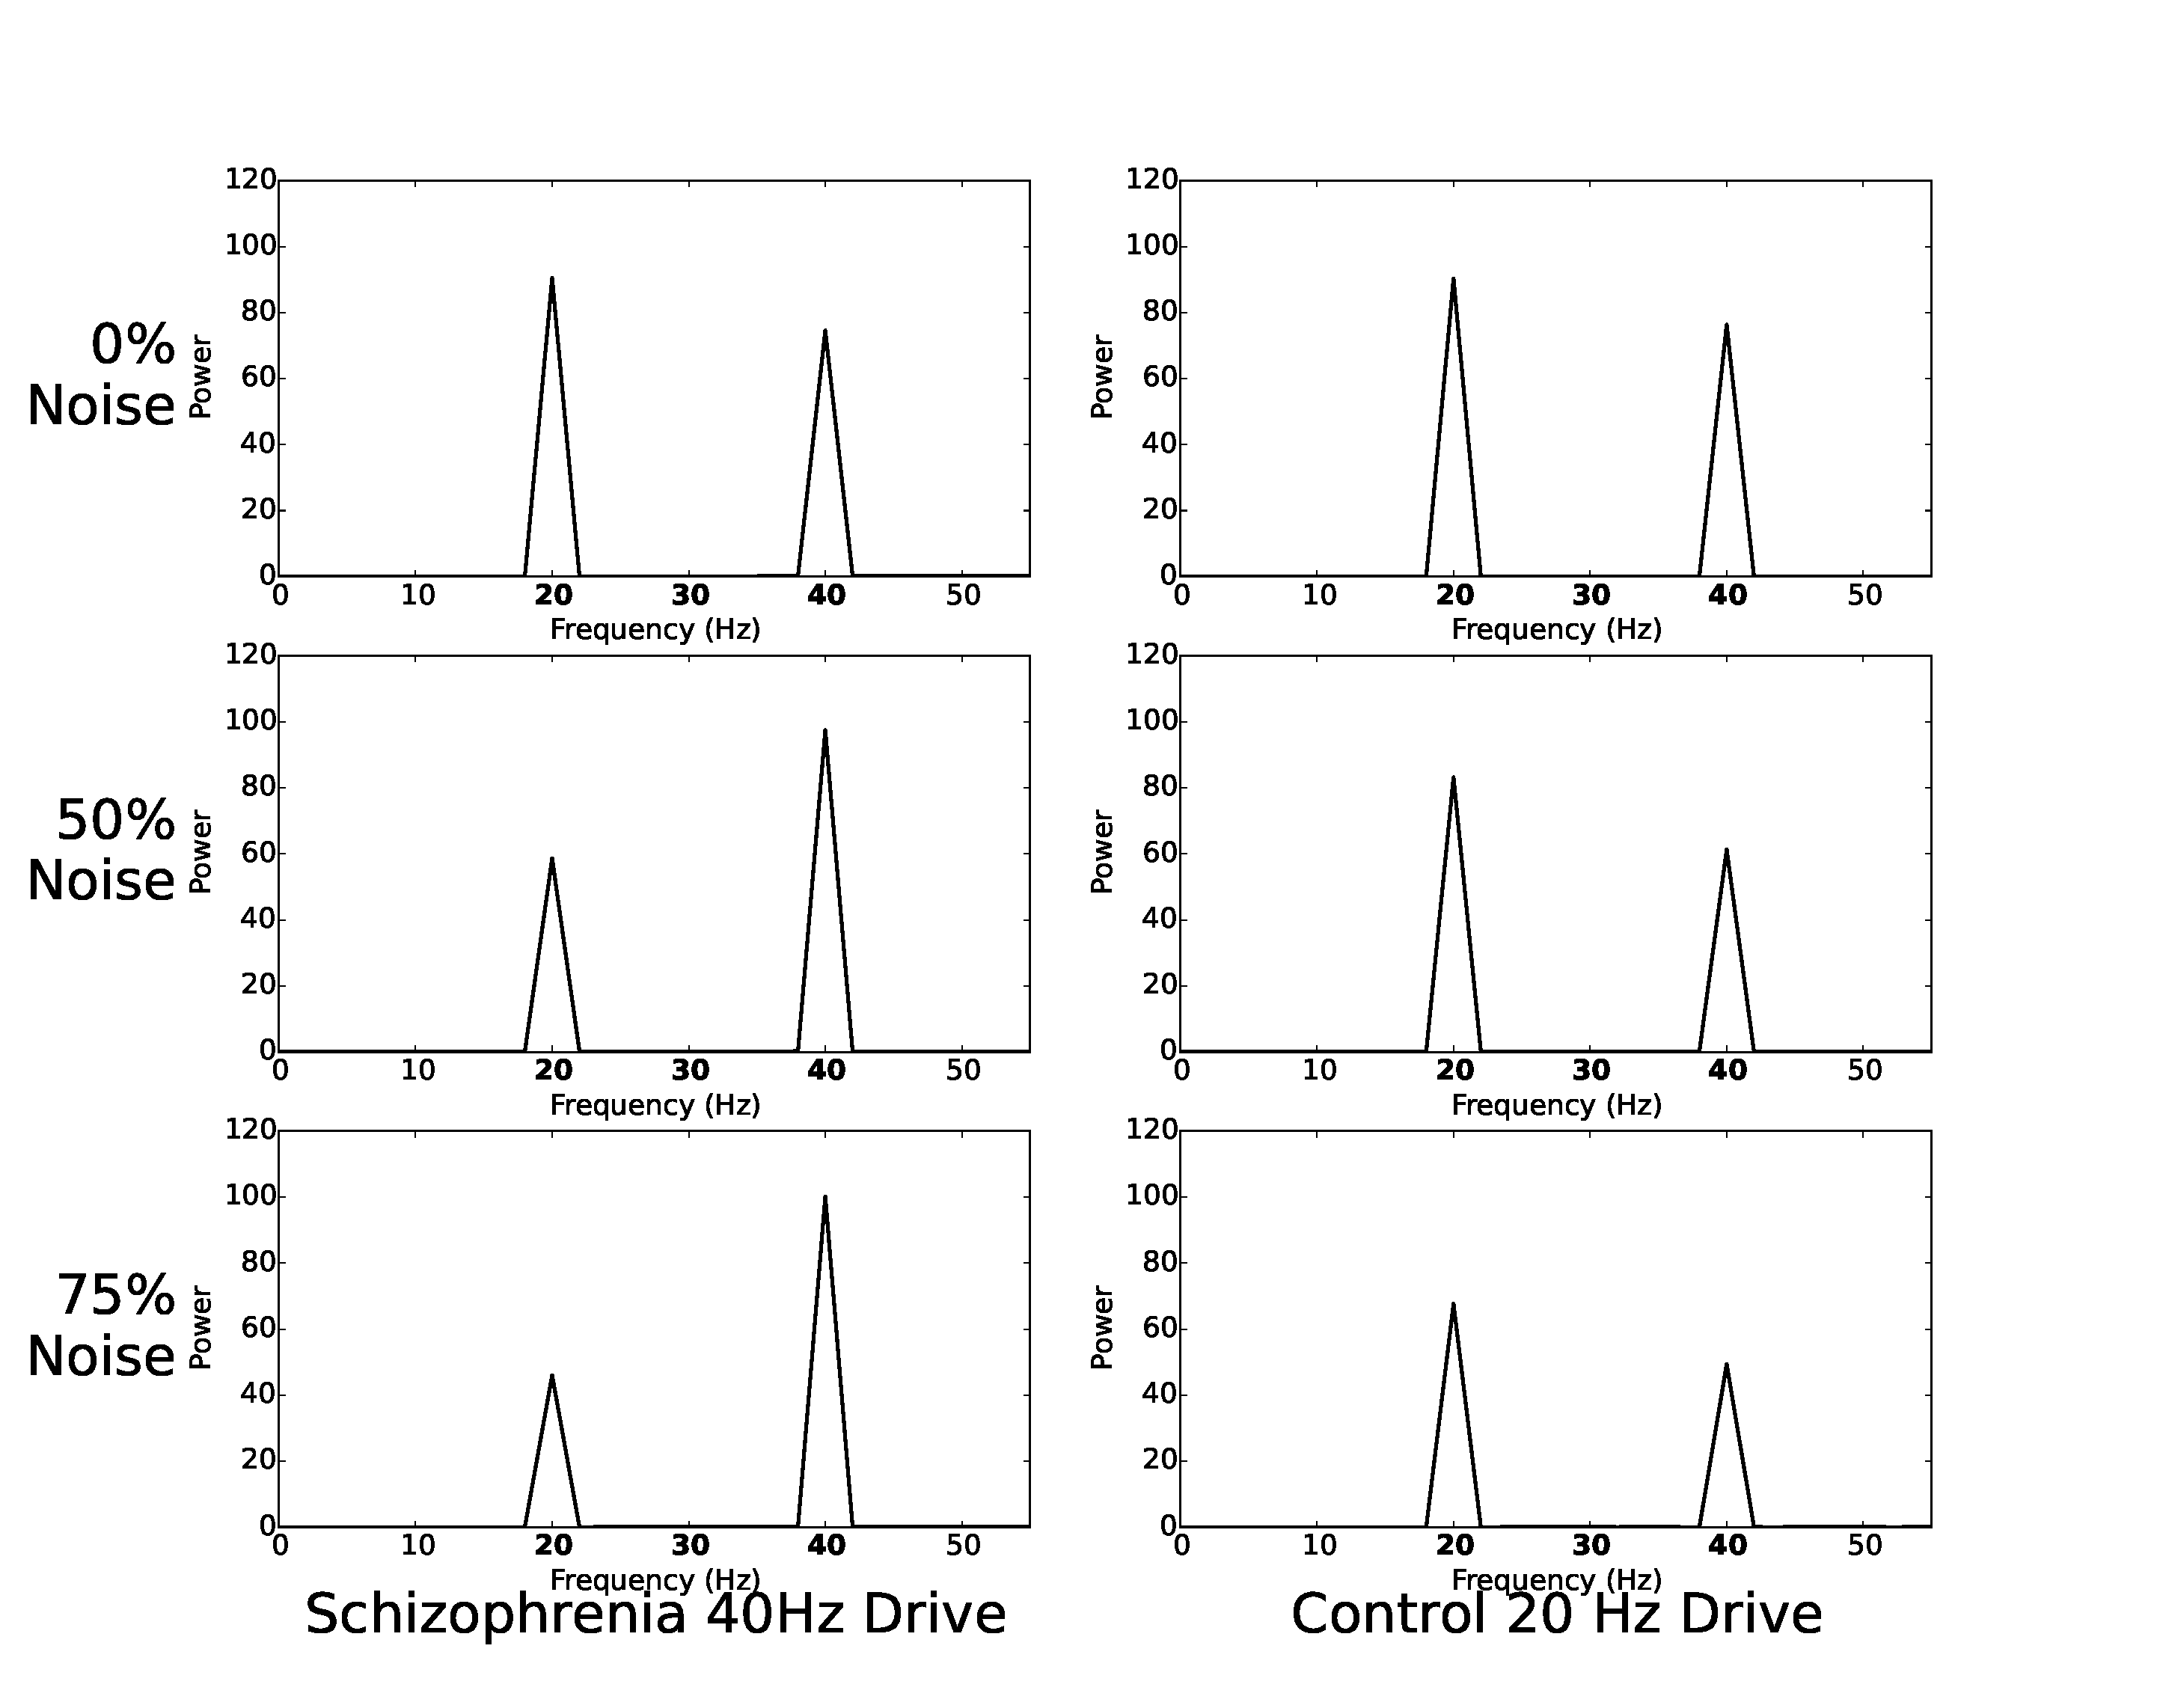
\includegraphics{Noise-Exploration-PSD.eps}
\caption{Replication of Figure 11: Single trial from the schizophrenia
network. 20 Hz drive. Network entrains to 20 Hz without 40 Hz component,
as can be seen in the frequency diagram, raster plot and MEG trace. note
that the 40 Hz power in the power spectrum is a
harmonic.}\label{fig:NoiseExplorationPSD}
\end{figure}


\FloatBarrier

\section{Conclusion}\label{conclusion}

Overall, we believe we have faithfully reproduced the main fetaures of
the simple model from \autocite{Vierling2008}. However, we note that
overall features a re a little bit less pronounced in our
reimplementation compared to the original model. We have explored possible explanations for this discrepancy
and conclude that it might come from minor inconsistencies with respect to parameters in the original model. Nevertheless,
the mechanism proposed in the original model could be reproduced and presents a possible explanation for deficits in 
auditory steady-state responses in patients suffering from schizophrenia.

{\sffamily \small
  \printbibliography[title=References]
}
\end{document}
